\documentclass[12pt]{article}
    % General document formatting
    \usepackage[margin=1in]{geometry}
    \usepackage[parfill]{parskip}
    \usepackage[utf8]{inputenc}
    \usepackage[T1]{fontenc}    
    % Set the font for the document
    \usepackage[scaled=1]{helvet}
    \renewcommand{\familydefault}{\sfdefault}    
    % Related to math
    \usepackage{amsmath,amssymb,amsfonts,amsthm}
    \usepackage{mathtools}
    % To set the mathematical font to helvetica as well
    \usepackage[helvet]{sfmath}
    \everymath={\sf}
    % To write differential equations in an easy way
    \usepackage{physics}
    % For referencing footnotes
    \usepackage[symbol]{footmisc}
    % To add links in the text
    \usepackage{url}
    % To add figures
    \usepackage{graphicx}
    % Set the graphics-path, i.e. where we store the figures
    \graphicspath{{./images/}}
    % To allow for greek letters in equation mode
    \usepackage{sansmathfonts}
    \usepackage{sansmath}
    \sansmath
    % To allow for alignment in tables
    \usepackage{tabularx}

% THE DOCUMENT BEGINS
\begin{document}

\begin{titlepage}
  \Large \textbf{Supplementary material for the article}\\[1cm]
  \Huge \textbf{Retiring Occam's razor in mechanistic modelling: the role of symmetries in model selection}\\[1cm]\normalsize

 \vspace{3.0cm}
        \setcounter{footnote}{1}
       Johannes Borgqvist\footnote{\label{Oxford}Wolfson Centre for Mathematical Biology, Mathematical Institute, University of Oxford, United Kingdom}\footnote{\label{WennerGren} Research fellow at the Wenner-Gren Foundations, Sweden}\footnote{\label{Linacre} Junior Research Fellow (JRF) at Linacre College, University of Oxford, United Kingdom}\footnote{E-mail: \url{Johannes.Borgqvist@maths.ox.ac.uk}} and Sam Palmer\footref{Oxford}.


  
\end{titlepage}

       \renewcommand*{\thefootnote}{\arabic{footnote}}
        \setcounter{footnote}{0}
\tableofcontents
\listoffigures
\listoftables
\newpage




\section{Finding the symmetries of the three candidate\\models}

The aim is to find the symmetries of three models predicting risk profiles over time. The focus of the article is the following three models \cite{Palmer1883}:

\begin{align}
R(t)&=Ae^{\alpha t},\label{eq:exp}\\
R(t)&=At^{\gamma},\label{eq:power_law}\\
R(t)&=\dfrac{A}{\exp\left(e^{-\alpha(t-\tau)}\right)-1}.\label{eq:mixed}
\end{align}
More precisely, the comparison in the main article is between \eqref{eq:power_law} and \eqref{eq:mixed} as these two models fit the data the best. Despite the fact that the model in \eqref{eq:exp} is excluded from the symmetry test due to its bad fit its symmetries are also calculated in this supplementary document. 

These models are referred to as the IM-I in \eqref{eq:exp}, the \textit{power law model} (PLM) in \eqref{eq:power_law} and the IM-II in \eqref{eq:mixed}. The idea is to use the symmetry based framework for model selection presented in \cite{ohlsson2020symmetry} on these models and the data presented in \cite{Palmer1883} in order to deduce which model that best predicts the risk profile. To this end, it is necessary to re-write these models as \textit{ordinary differential equations} (ODEs) and then solve the so called \textit{linearised symmetry condition} \cite{hydon2000symmetry} in order to find the symmetries of the models at hand. Subsequently, the ODE models will be derived, then the theory of symmetries of first order ODEs will be described briefly and then the symmetries for each of the three models will be derived.


\subsection{Derivation of the ODE models}
As symmetry methods are well-established for differential equations, it is advantageous to formulate the candidate models in this way. The corresponding ODE formulation of each model is derived by differentiating the curves in \eqref{eq:exp} to \eqref{eq:mixed} and then substituting the equation for the actual curve into the equation for the derivative. For \eqref{eq:exp}, we have

$$\dv{R}{t}=\dv{}{t}\left(Ae^{\alpha t}\right)=\alpha \underset{=R}{\underbrace{Ae^{\alpha t}}}=\alpha R$$
so
$$\dv{R}{t}=\alpha R.$$
For \eqref{eq:power_law}, we have
$$\dv{R}{t}=\dv{}{t}\left(At^{\gamma}\right)=\gamma A t^{\gamma-1}=\gamma\underset{=R}{\underbrace{\left(At^{\gamma}\right)}}t^{-1}=\gamma\dfrac{R}{t}$$
so
$$\dv{R}{t}=\gamma\dfrac{R}{t}.$$

Lastly, for \eqref{eq:mixed} we have


\begin{align*}
  \dv{R}{t}&=\dv{}{t}\left[A\left(\exp\left(e^{-\alpha(t-\tau)}\right)-1\right)^{-1}\right]\\
           &=-A\left(\exp\left(e^{-\alpha(t-\tau)}\right)-1\right)^{-2}\exp\left(e^{-\alpha(t-\tau)}\right)\left(-\alpha e^{-\alpha(t-\tau)}\right)\\            &=\dfrac{\alpha}{A}\underset{=R^2}{\underbrace{\left(\dfrac{A}{\exp\left(e^{-\alpha(t-\tau)}\right)-1}\right)^2}}\exp\left(e^{-\alpha(t-\tau)}\right)e^{-\alpha(t-\tau)}\\
  &=\dfrac{\alpha}{A}R^2e^{-\alpha(t-\tau)}\exp\left(e^{-\alpha(t-\tau)}\right)
\end{align*}
so
$$\dv{R}{t}=\dfrac{\alpha}{A}R^2e^{-\alpha(t-\tau)}\exp\left(e^{-\alpha(t-\tau)}\right).$$

An important classification of an ODE is whether or not it is autonomous. This term implies that there is no dependence on the variable, e.g. the time $t$, in the right hand side of the ODE. As can be seen by comparing the ODE formulations it is possible to conclude that the three candidate models are qualitatively different (Tab \ref{tab:ODEs}). This qualitative difference is reflected in the symmetries as a well-known symmetry that characterises the autonomous family of ODEs which is not a symmetry of non-autonomous ODEs is the famous \textit{translation symmetry} which will be described later in the text.

Throughout the text, the right hand side of the ODE will be denoted by $\omega(t,R)$ and this will be referred to as the \textit{reaction term}. More precisely, for the three models predicting the risk profiles the ODEs will be written on the following form:

\begin{equation}
\dv{R}{t}=\omega(t,R).
\label{eq:general_ODE}
\end{equation}

\begin{table}[htbp!]
\begin{center}
\caption[ODE formulations of the three models.]{\textit{ODE formulations of the three models}. In the three columns from left to right the following is presented: the original model, the ODE formulation of the model and the characterisation of the ODE as either autonomous or non-autonomous. }
\begin{tabular}{||c|c|c|c||}
  \hline\hline
 & & & \\
\textit{Model}  & \textit{Curve} & \textit{ODE} & \textit{Characterisation}\\
 & & & \\  
  \hline\hline
 & & & \\
IM-I & $R(t)=Ae^{\alpha t}$  & $\dv{R}{t}=\alpha R$ & Autonomous\\
 & & & \\
  \hline
 & & & \\
PLM & $R(t)=At^{\gamma}$  & $\dv{R}{t}=\gamma\frac{R}{t}$ & Non-autonomous\\
 & & & \\
  \hline
 & & & \\
IM-II & $R(t)=\dfrac{A}{\exp\left(e^{-\alpha(t-\tau)}\right)-1}$  & $\dv{R}{t}=\frac{\alpha}{A}R^2e^{-\alpha(t-\tau)}\exp\left(e^{-\alpha(t-\tau)}\right)$ & Non-autonomous\\
 & & & \\
  \hline\hline
  \end{tabular}
 \label{tab:ODEs}
\end{center}
\end{table}


Before the symmetries of the three models are derived, a brief presentation of the theory of symmetries are presented in order to properly define the involved concepts. 

\subsection{Mathematical theory of symmetries of a single first order ODE}
In order for the symmetry based model selection framework proposed in \cite{ohlsson2020symmetry} to work, it is necessary to find symmetries that are \textit{unique} to each model. Before these calculations are conducted, the notion of a symmetry as a mathematical object will be presented.  

A symmetry denoted by $\Gamma$ is an operator that maps a solution curve $\gamma=(t,R(t))$ to another solution curve $\hat{\gamma}=(\hat{t},\hat{R})$ \cite{hydon2000symmetry}. Mathematically, this can be expressed as follows: $\Gamma:\gamma\mapsto\hat{\gamma}$. A more rigorous definition of these operators requires the introduction of some notation. If $B=\left\{t\in\mathbb{R}\right\}\simeq\mathbb{R}$ denotes the so called \textit{base space} which is the space of the variable and $F=\left\{y(t)\in\mathbb{R}\right\}\simeq\mathbb{R}$ denotes the so called \textit{fibre} being the space of the dependent variable or the function then the solutions curves $\gamma=(t,R(t))$ reside in the so called \textit{total space} $E=B\times F\simeq\mathbb{R}^2$ being the product space of the two previously mentioned spaces. Now, a pointwise symmetry $\Gamma$ maps every point on a solution curve to another point on another solution curve which can be summarised as follows $\Gamma:E\mapsto E$. In the context of this article, we are interested in symmetries that are so called $\mathcal{C}^\infty$ diffeomorphisms (an isomorphism of smooth manifolds) which are parametrised by a single parameter $\epsilon$. In particular, this means that the symmetry is continuous in the parameter $\epsilon$, it is also invertible and it can be represented as a Taylor series around $\epsilon=0$ \cite{hydon2000symmetry}. From now on, when we say that we are looking for a symmetry it will be understood to be of this type, and we will denote these by

$$\Gamma (\epsilon):(t,R)\mapsto(\hat{t}(\epsilon),\hat{R}(\epsilon)).$$

Due to the continuity of these symmetries, it is possible to obtain a local description of their action.

The key for finding symmetries is the local representation of them in terms of their Taylor series. For a given symmetry $\Gamma (\epsilon):(t,R)\mapsto(\hat{t}(\epsilon),\hat{R}(\epsilon))$, the Taylor expansion of the transformed coordinates around $\epsilon=0$ is the following

\begin{align*}
\hat{t}(\epsilon)&=t+\xi(t,R)\epsilon+\mathcal{O}\left(\epsilon^2\right)\\
\hat{R}(\epsilon)&=t+\eta(t,R)\epsilon+\mathcal{O}\left(\epsilon^2\right)\\
\end{align*}
where
$$\xi(t,R)=\left.\dv{\hat{t}}{\epsilon}\right|_{\epsilon=0}\;\;\mathrm{and}\;\;\eta(t,R)=\left.\dv{\hat{R}}{\epsilon}\right|_{\epsilon=0}.$$
These latter two terms $\left(\xi,\eta\right)$ are referred to as the tangents of the symmetry and they define the vector field
\begin{equation}
  X=\xi(t,R)\partial t+\eta(t,R)\partial R
  \label{eq:generator}
\end{equation}

  
which is called the \textit{infinitesimal generator of the Lie group} as the set of symmetries form a one parameter Lie group \cite{hydon2000symmetry}. By defining the exponential map as follows

$$e^{\epsilon X}=\sum_{j=0}^{\infty}\frac{\epsilon^j}{j!}X^j$$
the symmetry $\Gamma:(t,R)\mapsto(\hat{t}(\epsilon),\hat{y}(\epsilon))$ is generated by the infinitesimal generator of the Lie group in the following manner
\begin{equation}
  \Gamma(\epsilon):(t,R)\mapsto\left(e^{\epsilon X}t,e^{\epsilon X}R\right).
  \label{eq:exp_map}
\end{equation}
In other words, it is enough to calculate the tangents to obtain the generator $X$ in \eqref{eq:generator} which subsequently can be used to obtain the symmetries through the exponential map according to \eqref{eq:exp_map}. Thus, the task of finding symmetries revolves around finding the tangents $\xi$ and $\eta$ in the infinitesimal generator of the Lie group $X$.

The tangents can be found by solving the \textit{linearised symmetry condition}. For a first order ODE \cite{hydon2000symmetry}, this condition corresponds to solving a two dimensional PDE which looks as follows:

\begin{equation}
  \pdv{\eta}{t}+\left(\pdv{\eta}{R}-\pdv{\xi}{t}\right)\omega(t,R)-\pdv{\xi}{R}\omega(t,R)^2=\xi\pdv{\omega}{t}+\eta\pdv{\omega}{R}.
  \label{eq:lin_sym}
\end{equation}
Again, $\omega$ corresponds to the reaction term of the ODE in question as in \eqref{eq:general_ODE}. So the tangents $(\xi,\eta)$ are found by solving the linearised symmetry condition in \eqref{eq:lin_sym}, and then the symmetries are obtained using the exponential map as in \eqref{eq:exp_map}. Furthermore, it is possible to classify the action of a symmetry in a similar way to the classification of the ODEs in terms of their qualitative behaviour (Tab \ref{tab:ODEs}). The reason why this classification is necessary is on account of the fact that symmetries that map solutions curves to \textit{different} solution curves are required for the model selection procedure to work.

The so called \textit{reduced characteristic} denoted by $\overline{Q}$ is used to classify symmetries. For a first order ODE, this is defined as follows: \cite{hydon2000symmetry}

\begin{equation}
\overline{Q}(X)=\left.\overline{Q}(t,R)\right|_{\xi,\eta\;\textrm{defined by}\;X}=\eta(t,R)-\omega(t,R)\xi(t,R).
\label{eq:Q}
\end{equation}
If $\overline{Q}(X)=0$ for a specific solution $\gamma=(t,R)$, the solution is \textit{trivial} under the action of the symmetry. This implies that the symmetry maps points along the \textit{same} solution curve. Moreover, if $\overline{Q}(X)\equiv 0$ then the symmetry itself is \textit{trivial} meaning that it does not transform any point for any solution curve (for an illustration of the geometrical interpretation of the characteristic see \cite{borgqvist2020phdthesis}). In order for the symmetry framework to work, we require at least one unique and \textit{non-trivial} symmetry for each model, i.e. $\overline{Q}(X)\neq 0$ for the particular symmetry $X$ at hand, meaning that points on a solution curve are transformed to points on \textit{another} solution curve for each model. Hence, after the linearised symmetry condition is solved for each of the three models, the calculated symmetries will be characterised using the reduced characteristic in \eqref{eq:Q}. 


\subsection{Derivation of the symmetries}
For the purpose of selecting a model, we are looking for three non-trivial symmetries $\Gamma_1(\epsilon),\Gamma_2(\epsilon)$ and $\Gamma_3(\epsilon)$ that are \textit{unique} to each of the candidate models in \eqref{eq:exp}, \eqref{eq:power_law} and \eqref{eq:mixed} respectively. Subsequently, the derivation of each of these three symmetries is presented in chronological order. 
%-------------------------------------------------------------------------------------------
% THE IM-I
%-------------------------------------------------------------------------------------------
\subsubsection{The IM-I}
For the sake of notation, let's denote the tangents in the infinitesimal generator of the Lie group for the IM-I by $\xi_3(t,R)$ and $\eta_3(t,R)$ respectively. The reaction term in \eqref{eq:exp} is given by $\omega_3(t,R)=\alpha R$. For the partial derivatives in the linearised symmetry condition, we have

$$\pdv{\omega_3}{t}=0,\;\;\pdv{\omega_3}{R}=\alpha\;\;\mathrm{and}\;\;\omega_3^2=\alpha^2R^2 .$$
Plugging in these expressions into \eqref{eq:lin_sym} yields
$$\pdv{\eta_3}{t}+\left(\pdv{\eta_3}{R}-\pdv{\xi_3}{t}\right)\alpha R-\pdv{\xi_3}{R}\alpha^2R^2=\eta_3\alpha$$
and by organising this as a polynomial in $R$, the above expression can be written as follows:
$$\left[\pdv{\eta_3}{t}-\alpha\eta_3\right]R^0+\left[\alpha\left(\pdv{\eta_3}{R}-\pdv{\xi_3}{t}\right)\right]R+\left[\alpha^2\pdv{\xi_3}{R}\right]R^2=0 .$$
Now, since the monomials $\left\{R^0,R^1,R^2\right\}$ in the above polynomial are linearly independent it follows that the following so called \textit{determining equations} \cite{hydon2000symmetry} must hold:
\begin{align}
  \pdv{\eta_3}{t}-\alpha\eta_3&=0,\label{eq:mod_1_det_1}\\
  \alpha\left(\pdv{\eta_3}{R}-\pdv{\xi_3}{t}\right)&=0,\label{eq:mod_1_det_2}\\
  \alpha^2\pdv{\xi_3}{R}&=0.\label{eq:mod_1_det_3}
\end{align}
From \eqref{eq:mod_1_det_1}, it follows that $\eta_3$ must be of the form
$$\eta_{3}(t,R)=C_1(R)e^{\alpha t} .$$
From \eqref{eq:mod_1_det_3}, it follows that that the tangent in the time direction is univariate implying that $\xi_3(t,R)=\xi_3(t)$. Plugging in these two expressions into \eqref{eq:mod_1_det_2} results in the following equation
$$C_1'(R)e^{\alpha t}=\pdv{\xi_3}{t}$$
and since $\xi_3$ is independent of $R$ it must hold that $C_1'(R)=C_2$ is a constant and hence
$$C_1(R)=C_2R+C_3$$
for two arbitrary constants $C_2,C_3$. Moreover, the solution to the above equation is given by the following calculations
\begin{align*}
  \pdv{\xi_3}{t}&=C_2e^{\alpha t}\\
  \Longrightarrow \xi_3(t)&=C_4+\dfrac{C_2}{\alpha}e^{\alpha t}
\end{align*}
for an additional arbitrary constant $C_4$. In summary, the tangents are given by
\begin{align*}
  \xi_3(t,R)&=C_4+\dfrac{C_2}{\alpha}e^{\alpha t},\\
  \eta_3(t,R)&= \left(C_2R+C_3\right)e^{\alpha t}.\\   
\end{align*}
Now, by plugging in these expressions into \eqref{eq:generator}, it is possible to organise the expressions according to the arbitrary constants $C_2,C_3$ and $C_4$ respectively. It follows that the most general infinitesimal generator of the Lie group $X_1$ for the IM-I in \eqref{eq:exp} is given by
\begin{align*}
  X_3&=\left(C_4+\dfrac{C_2}{\alpha}e^{\alpha t}\right)\partial_t+\left(\left(C_2R+C_3\right)e^{\alpha t}\right)\partial_R\\
   &=C_2\left[\underset{=X_{3,0}}{\underbrace{\frac{1}{\alpha}e^{\alpha t}\partial_t+Re^{\alpha t}\partial_R}}\right]+C_4\left[\underset{=X_{3,1}}{\underbrace{\partial_t}}\right]+C_3\left[\underset{=X_{3,2}}{\underbrace{e^{\alpha t}\partial_R}}\right]\\
     &=C_2X_{3,0}+C_4X_{3,1}+C_3X_{3,2},\\
  \Longrightarrow X_3&=C_2X_{3,0}+C_4X_{3,1}+C_3X_{3,2}.
\end{align*}
Note that the generator $X_3$ in fact corresponds to a set of generators. This set of generators is called the \textit{Lie Algebra} which is in fact a special type of vector space\footnote{A Lie Algebra is a vector space that is also equipped with an operation referred to as the Lie bracket and this type if vector space is closed under the Lie Bracket in addition to the standard requirements of a vector space.} \cite{hydon2000symmetry}. Thus, the set of generators is spanned by $\left\{X_{3,0},X_{3,1},X_{3,2}\right\}$ which forms a basis of the Lie algebra of the model in \eqref{eq:exp} and thus we have the following three generators to choose from:
\begin{align}
  X_{3,0}&=\frac{1}{\alpha}e^{\alpha t}\partial_t+Re^{\alpha t}\partial_R,\label{eq:mod_1_gen_1}\\
  X_{3,1}&=\partial_t,\label{eq:translation}\\
  X_{3,2}&=e^{\alpha t}\partial_R.\label{eq:mod_1_gen_2}
\end{align}
A non-trivial generator is chosen for the model selection procedure. Thus, each of these candidate generators are subsequently analysed by means of the reduced characteristic $\overline{Q}$ in \eqref{eq:Q}. For \eqref{eq:mod_1_gen_1}, the following holds
$$\overline{Q}(X_{3,0})=\eta_{3,0}-\omega_{3}\xi_{3,0}=Re^{\alpha t}-\left(\alpha R\right)\left(\frac{1}{\alpha}e^{\alpha t}\right)=0$$
and hence the generator $X_{3,0}$ is \textit{trivial}. For \eqref{eq:translation}, the following holds
$$\overline{Q}(X_{3,1})=\eta_{3,2}-\omega_{3}\xi_{3,2}=0-\left(\alpha R\right)\left(1\right)=-\alpha R\neq 0$$
and hence the generator $X_{3,1}$ is \textit{non-trivial}.  For \eqref{eq:mod_1_gen_2}, the following holds
$$\overline{Q}(X_{3,2})=\eta_{3,2}-\omega_{3}\xi_{3,2}=e^{\alpha t}-\left(\alpha R\right)\left(0\right)=e^{\alpha t}\neq 0$$
and hence the generator $X_{3,2}$ is \textit{non-trivial}. Thus, both symmetries stemming from the two non-trivial generators $X_{3,1}$ and $X_{3,2}$ will be calculated next. 


The generator $X_{3,1}$ is so well-known that it has a name and it is called the \textit{translation generator}. The reason why it is well-known is because it is common to all autonomous models. In order to find the corresponding symmetry, it is necessary to plug in the translation generator $X_{3,1}$ in \eqref{eq:translation} into the exponential map according to \eqref{eq:exp_map}.

For the transformed coordinate $\hat{t}(\epsilon)$, it is possible to apply the generator $X_{3,1}$ recursively on $t$. It follows that

\begin{align*}
X^{0}_{3,1}(t)&=t,\\  
X^{1}_{3,1}(t)&=\partial t(t)=1,\\
X^{2}_{3,1}(t)&=X_{3,1}(X_{3,1}(t))=X_{3,1}(1)=\partial t(1)=0,\\
X^{3}_{3,1}(t)&=X_{3,1}(X_{3,1}(t)^2)=X_{3,1}(0)=\partial t(0)=0,\\
&\vdots
\end{align*}
and thus it is only the first two terms in the exponential map that are non-zero. Note that the zeroth power of any generator corresponds to the trivial generator which leaves the point it transforms unchanged which is why the very first term satisfies $X^{0}_{3,1}(t)=t$. By \eqref{eq:exp_map}, it follows that
$$e^{\epsilon X_{3,1}}t=\sum_{j=0}^{\infty}\frac{\epsilon^j}{j!}X_{3,1}^j(t)=t+\epsilon.$$
Similarly, for the transformed coordinate $\hat{R}(\epsilon)$, the generator $X_{3,1}$ is applied recursively on $R$ which gives 
\begin{align*}
X^{0}_{3,1}(R)&=R,\\  
X^{1}_{3,1}(R)&=\partial t(R)=0,\\
X^{2}_{3,1}(R)&=X_{3,1}(X_{3,1}(R))=X_{3,1}(0)=\partial t(0)=0,\\
X^{3}_{3,1}(R)&=X_{3,1}(X_{3,1}(R)^2)=X_{3,1}(0)=\partial t(0)=0,\\
&\vdots
\end{align*}
and thus all terms are zero for this coordinate with the exception of the zeroth trivial term $X^{0}_{3,1}$. By \eqref{eq:exp_map}, the second coordinate is given by
$$e^{\epsilon X_{3,1}}R=\sum_{j=0}^{\infty}\frac{\epsilon^j}{j!}X_{3,1}^j(R)=R.$$
In conclusion, the translation symmetry $\Gamma_{3,1}(\epsilon)$ associated to the IM-I in \eqref{eq:exp} is given by
$$\Gamma_{3,1}(\epsilon):(t,R)\mapsto(t+\epsilon,R).$$
For most generators including the generator $X_{3,2}=e^{\alpha t}\partial R$, the corresponding symmetry is calculated by using a change of coordinates. More precisely, instead of calculating the symmetry using the exponential map it is beneficial to use a coordinate change from $(t,R)$ to, say, $(s,r)$ where the latter coordinates have the same properties as the translation generator in $X_{3,1}$. These coordinates are called the \textit{canonical coordinates} \cite{hydon2000symmetry} and they satisfy the following criteria
$$\Gamma_{3,2}:(s,r)\mapsto(s+\epsilon,r).$$
In other words, the transformed canonical coordinates satisfy $(\hat{s}(\epsilon),\hat{r}(\epsilon))=(s+\epsilon,r)$ which is equivalently formulated in terms of the infinitesimal generator of the Lie group by the equation $X_{3,2}=\partial_s$. The coordinate change from $(t,R)$ to $(s,r)$ is characterised by the following equations \cite{hydon2000symmetry}

\begin{align*}
\xi_{3,2}(t,R)\pdv{r}{t}+\eta_{3,2}(t,R)\pdv{r}{R}&=0,\\
\xi_{3,2}(t,R)\pdv{s}{t}+\eta_{3,2}(t,R)\pdv{s}{R}&=1.\\
\end{align*}
In the case of the generator $X_{3,2}$, the tangents are given by $(\xi_{3,2},\eta_{3,2})=\left(0,e^{\alpha t}\right)$ which results in the equations
\begin{align*}
e^{\alpha t}\pdv{r}{R}&=0,\\
e^{\alpha t}\pdv{s}{R}&=1.\\
\end{align*}
The solution to the first equation is that $r$ is a univariate function according to $r(t,R)=r(t)$ so we might as well choose $r=t$ implying that the symmetry will not move points in the $t$-direction which is in fact the case as $\xi_{3,2}=0$. The second equation yields the canonical coordinate
$$s=Re^{-\alpha t}=Re^{-\alpha r}.$$
By solving this equation for $R$ it follows that
$$R=se^{\alpha r}.$$
Now, the transformed coordinate $\hat{t}$ is defined in terms of the canonical coordinate $r$ as follows
$$\hat{t}(\epsilon)=\hat{r}(\epsilon)=r=t.$$
The transformed coordinate $\hat{R}$ is defined in terms of both canonical coordinates $s$ and $r$ and is given by the following calculations

\begin{align*}
  \hat{R}(\epsilon)&=\hat{s}(\epsilon)e^{\alpha \hat{r}(\epsilon)}\\
         &=\left(s+\epsilon\right)e^{\alpha r}\\
         &=\underset{=R}{\underbrace{se^{\alpha r}}}+\epsilon e^{\alpha r}=R+\epsilon e^{\alpha t}\\
    \Longrightarrow \hat{R}(\epsilon)&=R+\epsilon e^{\alpha t}.
\end{align*}
Consequently, the infinitesimal generator of the Lie group given by
$$X_{3,2}=e^{\alpha t}\partial R$$
generates the following non-trivial symmetry
$$\Gamma_{3,2}(\epsilon):(t,R)\mapsto (t,R+\epsilon e^{\alpha t}) .$$
%-------------------------------------------------------------------------------------------
% THE PLM
%-------------------------------------------------------------------------------------------
\subsubsection{The PLM}
Denote the tangents in the infinitesimal generator of the Lie group for the PLM by $\xi_1(t,R)$ and $\eta_1(t,R)$ respectively. The reaction term in \eqref{eq:exp} is given by

$$\omega_1(t,R)=\frac{\gamma R}{t} .$$

For the partial derivatives in the linearised symmetry condition, we have

$$\pdv{\omega_1}{t}=-\frac{\gamma R}{t^2},\;\;\pdv{\omega_1}{R}=\frac{\gamma}{t}\;\;\mathrm{and}\;\;\omega_1^2=\frac{\gamma^2 R^2}{t^2}.$$
Plugging in these derivatives into the linearised symmetry condition yields the following equation
$$\pdv{\eta_1}{t}+\left(\pdv{\eta_1}{R}-\pdv{\xi_1}{t}\right)\frac{\gamma R}{t}-\pdv{\xi_1}{R}\frac{\gamma^2 R^2}{t^2}=-\xi_1\frac{\gamma R}{t^2}+\eta_1\frac{\gamma}{t}$$
which can be organised according to the different powers of R
$$\left[\pdv{\eta_1}{t}-\eta_1\frac{\gamma}{t}\right]R^0+\left[\left(\pdv{\eta_1}{R}-\pdv{\xi_1}{t}\right)\frac{\gamma }{t}+\xi_1\frac{\gamma }{t^2}\right]R^1-\left[\pdv{\xi_1}{R}\frac{\gamma^2}{t^2}\right]R^2=0.$$
Since the monomials $\left\{R^0,R^1,R^2\right\}$ are linearly independent, the following determining equations must hold
\begin{align}
  \pdv{\eta_1}{t}-\eta_2\frac{\gamma}{t}&=0\label{eq:mod_2_det_1},\\
  \left(\pdv{\eta_1}{R}-\pdv{\xi_1}{t}\right)\frac{\gamma }{t}+\xi_1\frac{\gamma }{t^2}&=0\label{eq:mod_2_det_2},\\
\pdv{\xi_1}{R}\frac{\gamma^2}{t^2}&=0.\label{eq:mod_2_det_3}  
\end{align}
By \eqref{eq:mod_2_det_3}, the tangent $\xi$ is a univariate function of the variable $t$, i.e. $\xi(t,R)=\xi(t)$. By \eqref{eq:mod_2_det_1}, the following calculations hold

\begin{align*}
  \dv{\eta_1}{t}&=\dfrac{\gamma\eta_1}{t},\\
  \Longrightarrow \dfrac{\dd\eta_1}{\eta_1}&=\gamma\dfrac{\dd t}{t},\\
  \Longrightarrow \ln\left(\eta_1\right)&=\gamma\ln\left(t\right)+\tilde{C_1}(R)=\ln\left(t^\gamma\right)+\tilde{C_1}(R),\\
  \Longrightarrow \eta_1(t,R)&=\underset{=C_1(R)}{\underbrace{\exp\left(\tilde{C_1}(R)\right)}}t^\gamma=C_1(R)t^\gamma,                                                                         \end{align*}
where $C_1(R)$ is an arbitrary function of $R$. By plugging in these two expressions, into \eqref{eq:mod_2_det_2} the following equation must hold
$$\left(C_1'(R)t^\gamma-\pdv{\xi_1}{t}\right)\frac{\gamma }{t}+\xi_1\frac{\gamma }{t^2}=0.$$
and since $\xi_2$ is independent of $t$ it must follow that $C_1'(R)=C_2$ and $C_1(R)=C_2R+C_3$ for two arbitrary integration constants $C_2,C_3$. Moreover, the solution to the last ODE is given by the following calculations:


\begin{align*}
  C_2t^\gamma-\pdv{\xi_1}{t}+\frac{\xi_1 }{t}&=0\\
  \Longrightarrow \pdv{\xi_1}{t}&=\frac{\xi_1 }{t}+C_2t^\gamma\\
  \left\{\textrm{Multiply with integrating factor}:\;\;\exp(-\ln(t))=\dfrac{1}{\exp(\ln(t))}=\dfrac{1}{t}\right\}&\\
  \Longrightarrow \dfrac{1}{t}\pdv{\xi_1}{t}&=\frac{\xi_1 }{t^2}+C_2t^{\gamma-1}\\
  \Longrightarrow \dfrac{1}{t}\pdv{\xi_1}{t}-\frac{\xi_1 }{t^2}&=C_2t^{\gamma-1}\\
  \Longrightarrow \dv{}{t}\left(\dfrac{1}{t}\xi_1(t)\right)&=C_2t^{\gamma-1}\\
  \Longrightarrow \dfrac{1}{t}\xi_1(t)&=\int C_2t^{\gamma-1}\dd t=\dfrac{C_2}{\gamma}t^\gamma+C_4\\
  \Longrightarrow \xi_1(t)=\dfrac{C_2}{\gamma}t^{\gamma+1}+C_4t
\end{align*}
where $C_4$ is an additional arbitrary coefficient. Thus, the tangents for the model in \eqref{eq:power_law} are given by

\begin{align*}
\xi_1(t)&=\dfrac{C_2}{\gamma}t^{\gamma+1}+C_4t,\\
\eta_1(t,R)&=\left(C_2R+C_3\right)t^\gamma.  
\end{align*}
Similarly, as with the previous generator it is possible to organise the most general form of the infinitesimal generator of the Lie group $X_1$ for the PLM in \eqref{eq:power_law} with respect to the integration constants $C_2$, $C_3$ and $C_4$ respectively. This organisation is summarised in the following calculations
\begin{align*}
  X_1&=\left[\dfrac{C_2}{\gamma}t^{\gamma+1}+C_4t\right]\partial_t+\left[\left(C_2R+C_3\right)t^\gamma\right]\partial_R\\
     &=C_2\left[\underset{=X_{1,0}}{\underbrace{\dfrac{t^{\gamma+1}}{\gamma}\partial_t+Rt^{\gamma}\partial_R}}\right]+C_4\left[\underset{=X_{1,1}}{\underbrace{t\partial_t}}\right]+C_3\left[\underset{X_{1,2}}{\underbrace{t^{\gamma}\partial_R}}\right]\\
&=C_2X_{1,0}+C_4X_{1,1}+C_3X_{1,2}.
\end{align*}
In similarity with the previous model, the Lie algebra of the PLM in \eqref{eq:power_law} is spanned by the set of basis generators $\left\{X_{2,1},X_{2,2},X_{2,3}\right\}$ listed below
\begin{align*}
  X_{1,0}&=\dfrac{t^{\gamma+1}}{\gamma}\partial_t+Rt^{\gamma}\partial_R,\\
  X_{1,1}&=t\partial_t,\\
  X_{1,2}&=t^{\gamma}\partial_R.\\
\end{align*}
Similarly as before, these three generators will now be classified as either trivial or non-trivial. For the first generator, the reduced characteristic $\overline{Q}$ in \eqref{eq:Q} is given by
$$\overline{Q}(X_{1,0})=\eta_{1,0}-\omega_1\xi_{1,0}=Rt^{\gamma}-\left(\dfrac{\gamma R}{t}\right)\left(\dfrac{t^{\gamma+1}}{\gamma}\right)=0$$
and hence the generator $X_{1,0}$ is trivial. For the second generator, it follows that
$$\overline{Q}(X_{1,1})=\eta_{1,1}-\omega_1\xi_{1,1}=0-\left(\dfrac{\gamma R}{t}\right)\left(t\right)=\gamma R\neq 0$$
and hence the generator $X_{1,1}$ is non-trivial. For the third generator, it follows that
$$\overline{Q}(X_{1,2})=\eta_{1,2}-\omega_1\xi_{1,2}=t^{\gamma}-\left(\dfrac{\gamma R}{t}\right)\left(0\right)=t^{\gamma}\neq 0$$
and hence the generator $X_{1,2}$ is non-trivial.  Thus, the symmetries generated by $X_{1,1}$ and $X_{1,2}$ respectively will be calculated next.

Just as the translation generator, the generator $X_{1,1}=t\partial t$ has a name which is the \textit{scaling generator}. Its symmetry can be calculated using the exponential map as in \eqref{eq:exp_map}. By applying the generator recursively to $t$, it follows that

\begin{align*}
  X^{0}_{1,1}(t)&=t\\
  X^{1}_{1,1}(t)&=t\underset{=1}{\underbrace{\partial_t(t)}}=t\\
  X^{2}_{1,1}(t)&=X_{1,1}(\underset{=t}{\underbrace{X_{1,1}(t)}})=t\\
  X^{3}_{1,1}(t)&=X_{1,1}(\underset{=t}{\underbrace{X^{2}_{1,1}(t)}})=t\\  
  &\vdots
\end{align*}
and hence all terms in the exponential map equals $t$ for the scaling generator. Thus, it follows that the transformed coordinate is given by
$$e^{\epsilon X_{1,1}}t=\sum_{j=0}^{\infty}\frac{\epsilon^j}{j!}\underset{=t}{\underbrace{X_{1,1}^j(t)}}=t\underset{=e^{\epsilon}}{\underbrace{\sum_{j=0}^{\infty}\frac{\epsilon^j}{j!}}}=te^{\epsilon}.$$
The $R$-coordinate is unaffected by the action of the symmetry implying that
$$e^{\epsilon X_{1,1}}R=R$$
and hence the \textit{scaling symmetry} $\Gamma_{2,3}$ is given by
$$\Gamma_{1,1}(\epsilon):(t,R)\mapsto \left(te^{\epsilon},R\right).$$
To calculate the symmetry generated by $X_{1,2}=t^{\gamma}\partial_R$, the method based on the canonical coordinates will be used. Note that for this generator, the tangents are given by $\xi_{1,2}=0$ and $\eta_{1,2}=t^{\gamma}$ respectively and the canonical coordinates $(s,r)$ satisfy the following equations

\begin{align*}
\xi_{1,2}(t,R)\pdv{r}{t}+\eta_{1,2}(t,R)\pdv{r}{R}&=0,\\
\xi_{1,2}(t,R)\pdv{s}{t}+\eta_{1,2}(t,R)\pdv{s}{R}&=1.\\
\end{align*}
By plugging in the tangents $\xi_{1,2}$ and $\eta_{1,2}$, these equation become
\begin{align*}
t^{\gamma}\pdv{r}{R}&=0,\\
t^{\gamma}\pdv{s}{R}&=1.\\
\end{align*}
By the same arguments as for the previous model, since the generator $X_{1,2}$ does not transform points in the $t$-direction the second canonical coordinate is set to $r=t$. Consequently, the transformed coordinate for $t$ is given by
$$\hat{t}(\epsilon)=\hat{r}(\epsilon)=r=t.$$
The first canonical coordinate is given by
$$s=\dfrac{R}{t^{\gamma}}$$
and solving this equation for $R$ as well as re-writing the equation in terms of the canonical coordinates yields
$$R=st^{\gamma}=sr^{\gamma}.$$
Lastly, the transformed coordinate for $R$ is given by
$$\hat{R}(\epsilon)=\hat{s}(\epsilon)\hat{r}(\epsilon)^{\gamma}=(s+\epsilon)r^{\gamma}=\underset{=R}{\underbrace{sr^{\gamma}}}+\epsilon r^{\gamma}=R+\epsilon t^{\gamma}.$$
In summary, the infinitesimal generator of the Lie group generated by $X_{2,2}=t^{\gamma}\partial_R$ generates the following symmetry
$$\Gamma_{1,2}(\epsilon):(t,R)\mapsto (t,R+\epsilon t^{\gamma}).$$
%-------------------------------------------------------------------------------------------
% THE IM-II
%-------------------------------------------------------------------------------------------
\subsubsection{The IM-II}
Denote the tangents of the IM-II by $\xi_{2}(t,R)$ and $\eta_{2}(t,R)$ respectively. The reaction term for this model is given by

$$\omega_2(t,R)=\frac{\alpha}{A}R^2e^{-\alpha(t-\tau)}\exp\left(e^{-\alpha(t-\tau)}\right)$$
and the linearised symmetry condition is given by
$$\pdv{\eta_2}{t}+\left(\pdv{\eta_2}{R}-\pdv{\xi_2}{t}\right)\omega_2-\pdv{\eta_2}{t}\omega_2^2=\xi_3\pdv{\omega_2}{t}+\eta_3\pdv{\omega_2}{R}.$$
Thus, the task at hand is to calculate the three terms $\omega_2^2$, $\partial\omega_2/\partial t$ and $\partial\omega_2/\partial R$ in order to plug these expressions into the linearised symmetry condition above. For the quadratic term, it follows that the middle factor satisfies
$$\left(\exp\left(e^{-\alpha(t-\tau)}\right)\right)^2=\exp\left(e^{-\alpha(t-\tau)}\right)\exp\left(e^{-\alpha(t-\tau)}\right)=\exp\left(2e^{-\alpha(t-\tau)}\right)$$
and hence the quadratic term is given by
$$\omega_2^2=\dfrac{\alpha^2}{A^2}R^4e^{-2\alpha(t-\tau)}\exp\left(2e^{-\alpha(t-\tau)}\right).$$
For the time derivative, it follows that
\begin{align*}
  \pdv{\omega_2}{t}&=\pdv{}{t}\left[\dfrac{\alpha}{A}e^{-\alpha(t-\tau)}\exp\left(e^{-\alpha(t-\tau)}\right)R^2\right]\\
  &=\dfrac{\alpha R^2}{A}\left[-\alpha e^{-\alpha(t-\tau)}\exp\left(e^{-\alpha(t-\tau)}\right)+e^{-\alpha(t-\tau)}\exp\left(e^{-\alpha(t-\tau)}\right)-\alpha e^{-\alpha(t-\tau)}\right]\\
  &=-\dfrac{\alpha^2R^2}{A}\left[e^{-\alpha(t-\tau)}\exp\left(e^{-\alpha(t-\tau)}\right)+e^{-2\alpha(t-\tau)}\exp\left(e^{-\alpha(t-\tau)}\right)\right]
\end{align*}
holds. For the derivative with respect to $R$, we have
$$\pdv{\omega_2}{R}=2\dfrac{\alpha}{A}e^{-\alpha(t-\tau)}\exp\left(e^{-\alpha(t-\tau)}\right)R.$$
Now, plugging in these expressions into the linearised symmetry condition leads to the following equation
\begin{align*} \pdv{\eta_2}{t}&+\left(\pdv{\eta_2}{R}-\pdv{\xi_2}{t}\right)\left[\frac{\alpha}{A}R^2e^{-\alpha(t-\tau)}\exp\left(e^{-\alpha(t-\tau)}\right)\right]-\pdv{\xi_2}{R}\left[\dfrac{\alpha^2}{A^2}R^4e^{-2\alpha(t-\tau)}\exp\left(2e^{-\alpha(t-\tau)}\right)\right]\\ &=\xi_2\left(-\dfrac{\alpha^2R^2}{A}\left[e^{-\alpha(t-\tau)}\exp\left(e^{-\alpha(t-\tau)}\right)+e^{-2\alpha(t-\tau)}\exp\left(e^{-\alpha(t-\tau)}\right)\right]\right)\\
  &+\eta_2\left(2\dfrac{\alpha}{A}e^{-\alpha(t-\tau)}\exp\left(e^{-\alpha(t-\tau)}\right)R\right).
\end{align*}
Since the monomials $\left\{R^0,R^1,R^2,R^4\right\}$ are \textit{linearly independent}, it follows that the following four equations must hold
\begin{align}
  R^{0}:&\;\;\;\;\;\pdv{\eta_2}{t}=0,\label{eq:3_1}\\
  R^{1}:&\;\;\;\;\;2\eta_2\dfrac{\alpha}{A}e^{-\alpha(t-\tau)}\exp\left(e^{-\alpha(t-\tau)}\right)=0,\label{eq:3_2}\\ R^{2}:&\;\;\;\;\;\dfrac{\alpha}{A}e^{-\alpha(t-\tau)}\exp\left(e^{-\alpha(t-\tau)}\right)\left[\left(\pdv{\eta_2}{R}-\pdv{\xi_2}{t}\right)+\alpha\xi_2\left(1+e^{-\alpha(t-\tau)}\right)\right]=0,\label{eq:3_3}\\
R^{4}:&\;\;\;\;\; \left[\dfrac{\alpha^2}{A^2}e^{-2\alpha(t-\tau)}\exp\left(2e^{-\alpha(t-\tau)}\right)\right]\pdv{\xi_2}{R}=0.\label{eq:3_4} 
\end{align}
The tangent in the $R$-direction $\eta_2$ must satisfy $\eta_2=0$ according to \eqref{eq:3_1} and \eqref{eq:3_2}. Moreover, the tangent in the $t$-direction must be a univariate function of $t$, i.e. $\xi_2(t,R)=\xi_2(t)$, as it follows that $\partial\xi_2/\partial R=0$ according to \eqref{eq:3_4}. Lastly, tangent $\xi_2$ in the $t$-direction must satisfy the following ODE
$$\dv{\xi_2}{t}=\alpha\xi_2\left(1+e^{-\alpha(t-\tau)}\right)$$
according to \eqref{eq:3_3}. Now, by defining the function $f(t)=\alpha\left(1+e^{-\alpha(t-\tau)}\right)$ its primitive function is
$$F(t)=\alpha t-e^{-\alpha(t-\tau)}.$$
Thus, by multiplying the above ODE with the integrating factor ``$\exp\left(-F(t)\right)$'', the resulting equation is
$$\underset{=\pdv{}{t}\left(\exp\left(-F(t)\right)\xi_2\right)\left\{=\exp\left(-F(t)\right)\dv{\xi_2}{t}+\dv{\exp\left(-F(t)\right)}{t}\xi_2\right\}}{\underbrace{\exp\left(-\left(\alpha t-e^{-\alpha(t-\tau)}\right)\right)\dv{\xi_2}{t}-\underset{=-\pdv{\exp\left(-F(t)\right)}{t}}{\underbrace{\exp\left(-\left(\alpha t-e^{-\alpha(t-\tau)}\right)\right)\alpha\left(1+e^{-\alpha(t-\tau)}\right)}}\xi_2}}=0$$
which can be re-written by using the product rule as follows
$$\pdv{}{t}\left(\exp\left(-\left(\alpha t-e^{-\alpha(t-\tau)}\right)\right)\xi_2\right)=0.$$
Finally, by integrating with respect to $t$ the tangent is given by
$$\xi_2(t)=C_1\exp\left(\left(\alpha t-e^{-\alpha(t-\tau)}\right)\right)=C_1e^{\alpha t}\exp\left(-e^{-\alpha(t-\tau)}\right)$$
for an arbitrary integration constant $C_1$. Hence, the generator for the IM-II is given by
$$X_2=e^{\alpha t}\exp\left(-e^{-\alpha(t-\tau)}\right)\partial_t.$$
The generator is non-trivial as
\begin{align*}
  \overline{Q}(X_2)&=\eta_2-\omega_2\xi_2=0-\left[\frac{\alpha}{A}R^2e^{-\alpha(t-\tau)}\exp\left(e^{-\alpha(t-\tau)}\right)\right]\left[e^{\alpha t}\exp\left(-e^{-\alpha(t-\tau)}\right)\right]\\
  &=\frac{\alpha}{A}R^2e^{\alpha\tau}\neq 0.
\end{align*}

To calculate the symmetry $\Gamma_2$ generated by the infinitesimal generator of the Lie group $X_2$, the approach based on the canonical coordinates is used. For the generator $X_2$, the tangents are given by
$$\left(\xi_2,\eta_2\right)=\left(e^{\alpha t}\exp\left(-e^{-\alpha(t-\tau)}\right),0\right).$$
The canical coordinates $(s,r)$ satisfy the following equations 
\begin{align*}
\xi_{2}(t,R)\pdv{r}{t}+\eta_{2}(t,R)\pdv{r}{R}&=0,\\
\xi_{2}(t,R)\pdv{s}{t}+\eta_{2}(t,R)\pdv{s}{R}&=1,\\
\end{align*}
which by plugging in the tangents $\left(\xi_2,\eta_2\right)$ results in the following equations
\begin{align*}
e^{\alpha t}\exp\left(-e^{-\alpha(t-\tau)}\right)\pdv{r}{t}&=0,\\
e^{\alpha t}\exp\left(-e^{-\alpha(t-\tau)}\right)\pdv{s}{t}&=1.\\
\end{align*}
Since the generator $X_2$ is unidirectional in the sense that it only moves points in the $t$-direction and as $\partial r/\partial t=0$ we can set $r=R$. From the second equation, it follows that
\begin{align*}
  s&=\int e^{-\alpha t}\exp\left(e^{-\alpha(t-\tau)}\right)\dd t\\
&=-\dfrac{1}{\alpha e^{\alpha\tau}}\int \underset{\dv{e^{-\alpha t}}{t}}{\underbrace{\left(-\alpha e^{-\alpha t}\right)}}\underset{\textrm{Outer derivative}}{\underbrace{\left(e^{\alpha\tau}\exp\left(e^{\alpha\tau}e^{-\alpha t}\right)\right)}}\dd t\\
\{\textrm{Chain rule}\}\Longrightarrow&= -\dfrac{1}{\alpha e^{\alpha\tau}}\int \dv{}{t}\left(\exp\left(e^{\alpha\tau}e^{-\alpha t}\right)\right)\dd t\\
  \Longrightarrow s&=-\dfrac{e^{-\alpha\tau}\exp\left(e^{-\alpha(t-\tau)}\right)}{\alpha}.
\end{align*}
In order to be able to take the logarithm of the above expression, we must work with the absolute value as taking the logarithm is only allowed on positive expressions. Therefore, the value of $t$ is calculated in the following steps


\begin{align*}
  s&= -\dfrac{e^{-\alpha\tau}\exp\left(e^{-\alpha (t-\tau)}\right)}{\alpha}\\
  \Longrightarrow -\alpha e^{\alpha\tau} s&=\exp\left(e^{-\alpha (t-\tau)}\right)\\
  \Longrightarrow |\alpha e^{\alpha\tau} s|&=\exp\left(e^{-\alpha (t-\tau)}\right)\\
  \Longrightarrow -\alpha (t-\tau)&=\ln\left(\ln\left(|\alpha e^{\alpha\tau} s|\right)\right)\\
  \Longrightarrow t&=\tau-\dfrac{\ln\left(\ln\left(|\alpha e^{\alpha\tau} s|\right)\right)}{\alpha}. 
\end{align*}
Now, using this last equation, the transformed coordinate $\hat{t}$ is given by
\begin{align*}
  \hat{t}&=\tau-\dfrac{\ln\left(\ln\left(|\alpha e^{\alpha\tau} \hat{s}|\right)\right)}{\alpha}\\
         &=\tau-\dfrac{\ln\left(\ln\left(\left|\alpha e^{\alpha\tau} (s+\epsilon)\right|\right)\right)}{\alpha}\\
         &=\tau-\dfrac{\ln\left(\ln\left(\left|\alpha e^{\alpha\tau} \epsilon-\exp\left(e^{-\alpha (t-\tau)}\right)\right|\right)\right)}{\alpha}.\\  
\end{align*}
Consequently, the infinitesimal generator of the Lie group denoted by $X_2$ generates the following symmetry
$$\Gamma_2(\epsilon):(t,R)\mapsto\left(\tau-\dfrac{\ln\left(\ln\left(\left|\alpha e^{\alpha\tau} \epsilon-\exp\left(e^{-\alpha (t-\tau)}\right)\right|\right)\right)}{\alpha},R\right).$$
Note that the value $\epsilon=0$ indeed corresponds to the trivial symmetry as $\Gamma_2(0):(t,R)\mapsto(t,R)$ which is a required property of any symmetry.

\section{Summary of the calculated symmetries}

In the article, the symmetries of the IM-I is omitted as its fit is much worse than the other two candidate models. Although, the emphasis is on the comparison between the PLM and the IM-II the symmetries of the IM-I have also been calculated. A summary of all the calculated symmetries is presented below (Tab \ref{tab:sym_tab}).


\begin{table}[htbp!]
\begin{center}
\caption[Summary of the symmetries]{\textbf{Summary of the symmetries}. The models, their generators and the non-trivial symmetries are presented from left to right. }
\begin{tabular}{||c|c|c||}
\hline\hline
 & & \\
\textit{Model} & Generators & Non-trivial\\
& & Symmetries\\
& & \\
 \hline\hline
& & \\
PLM & $X_{1,0}=\left(\frac{t^{\gamma+1}}{\gamma}\right)\partial_t+Rt^{\gamma}\partial_R$& \\
  & $X_{1,1}=t\partial_t$& $\Gamma_{1,1}(\epsilon):(t,R)\mapsto \left(te^{\epsilon},R\right)$\\
  & $X_{1,2}=t^{\gamma}\partial_R$ & $\Gamma_{1,2}(\epsilon):(t,R)\mapsto (t,R+\epsilon t^{\gamma})$\\
 & & \\
 \hline
 & & \\
 IM-II & $X_2=e^{\alpha t}\exp\left(-e^{-\alpha(t-\tau)}\right)\partial_t$ & $\Gamma_2(\epsilon):(t,R)\mapsto\left(\tau-\dfrac{\ln\left(\ln\left(\left|\alpha e^{\alpha\tau}\epsilon-\exp\left(e^{-\alpha (t-\tau)}\right)\right|\right)\right)}{\alpha},R\right)$\\
 & & \\
 \hline
 & & \\
 IM-I & $X_{3,0}=\frac{1}{\alpha}e^{\alpha t}\partial_t+Re^{\alpha t}\partial_R$& \\
 & $X_{3,1}=\partial_t$& $\Gamma_{3,1}(\epsilon):(t,R)\mapsto(t+\epsilon,R)$\\
 & $X_{3,2}=e^{\alpha t}\partial R$& $\Gamma_{3,2}:(t,R)\mapsto (t,R+\epsilon e^{\alpha t}) $\\
 & & \\
 \hline\hline
 \end{tabular}
\label{tab:sym_tab}
\end{center}
\end{table}



A commonality between the three models is that all non-trivial generators are uni-directional. Both the PLM and the IM-I have $R$-directional symmetries, i.e. $\Gamma_{1,2}$ and $\Gamma_{3,2}$ whereas the IM-II
 merely has a $t$-directional symmetry in $\Gamma_{2}$. The action of the non-trivial symmetries of the PLM (Fig \ref{fig:PLM}), the IM-II (Fig \ref{fig:IM-II}) and the IM-I (Fig \ref{fig:IM-I}) respectively is illustrated below.

\begin{figure}[htbp!]
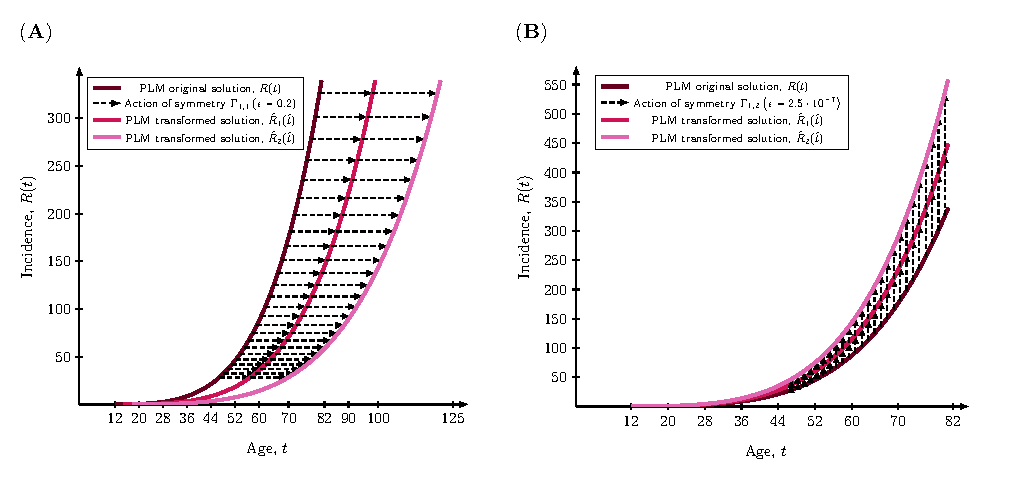
\includegraphics[width=\textwidth]{FigS2.pdf}
\caption[Action of the non-trivial symmetries of the PLM]{\textit{Action of the non-trivial symmetries of the PLM}. The original curve which is generated from the PLM with parameters $(A,\gamma)=(7.742,4.528)$ is transformed twice with the two non-trivial symmetries of the PLM. (\textbf{A}) The $t$-directional scaling symmetry $\Gamma_{1,1}$ with transformation parameter $\epsilon=0.2$. (\textbf{B}) The $R$-directional symmetry $\Gamma_{1,2}$ with transformation parameter $\epsilon=2.5\cdot 10^{-7}$.}
\label{fig:PLM}
\end{figure}

\begin{figure}[htbp!]
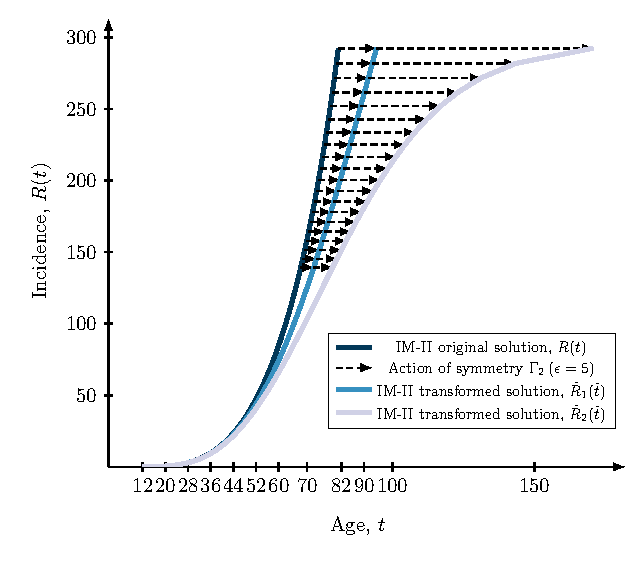
\includegraphics[width=\textwidth]{FigS3.pdf}
\caption[Action of the non-trivial symmetry of the IM-II]{\textit{Action of the non-trivial symmetry of the IM-II}. The original curve which is generated from the IM-II with parameters $(A,\tau,\alpha)=(130.721,58.378,0.044)$ is transformed twice with the non-trivial symmetry of the IM-II. More precisely, the original curve is transformed twice with the $t$-directional symmetry $\Gamma_{2}$ with transformation parameter $\epsilon=5$.}
\label{fig:IM-II}
\end{figure}




\begin{figure}[htbp!]
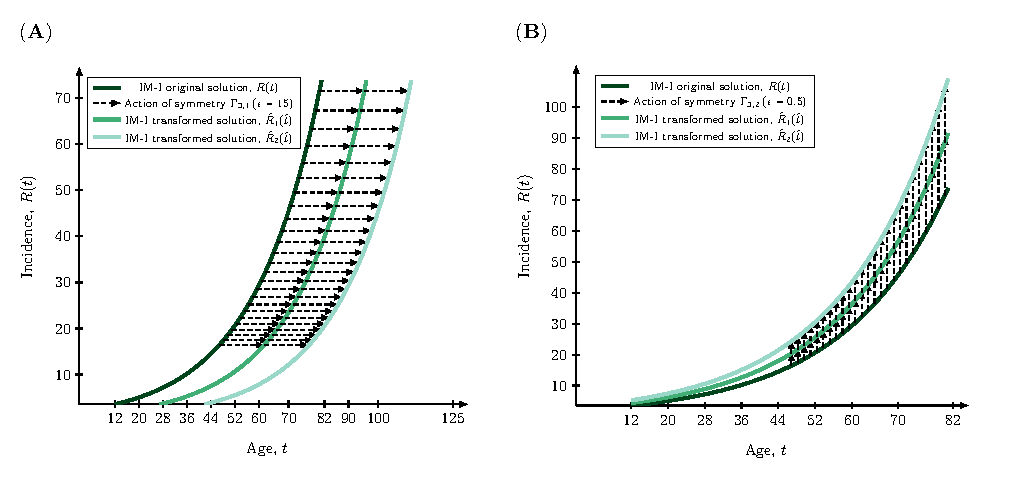
\includegraphics[width=\textwidth]{FigS1.pdf}
\caption[Action of the non-trivial symmetries of the IM-I]{\textit{Action of the non-trivial symmetries of the IM-I}. The original curve which is generated from the IM-I with parameters $(A,\alpha)=(2.090,0.044)$ is transformed twice with the two non-trivial symmetries of the PLM. (\textbf{A}) The $t$-directional translation symmetry $\Gamma_{3,1}$ with transformation parameter $\epsilon=15$. (\textbf{B}) The $R$-directional symmetry $\Gamma_{3,2}$ with transformation parameter $\epsilon=0.5$.}
\label{fig:IM-I}
\end{figure}

\section{Processing of the data and the curve fitting}

In order to conduct the curve fitting, the data is processed in two steps (Fig \ref{fig:data_processing}). The data in this cas e is a time series containing the age of the subjects denoted by $t$ and the number of incidences of colon cancer as a function of the age denoted by $R(t)$. As the number of incidences of colon cancer is zero below the ages of 12 years, the first 12 data points are removed in the time series. In addition, the fitting to the data is conducted on the logarithm of the incidences, i.e. the models are fitted to a modified time series containing ages $t$ versus the logarithm of the incidences $\ln\left(R(t)\right)$. Provided the fact that it is the logarithm of the incidences that are reported, it is necessary to fit the logarithmic version of the models. 


\begin{figure}[htbp!]
  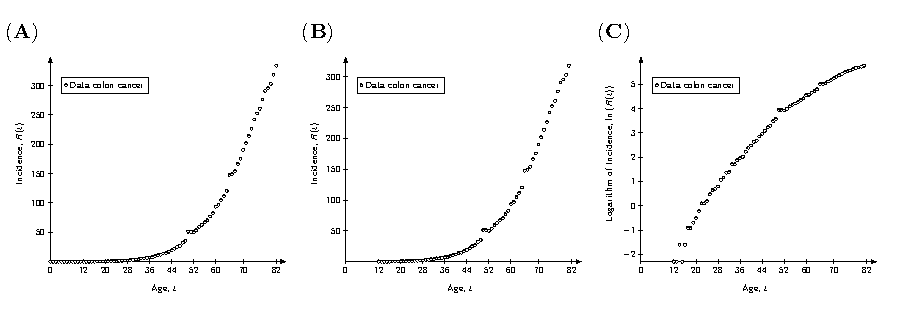
\includegraphics[width=\textwidth]{FigS4.pdf}
  \caption[Processing of the data]{\textit{Processing of the data}. The processing of the original data in (\textbf{A}) is conducted in two steps. (\textbf{B}) Remove all zero incidences corresponding to all ages below 12 years. More precisely, this corresponds to the removal of the first 12 data points in the original time series. (\textbf{C}) Apply the logarithm to the incidences so that $\ln\left(R(t)\right)$ is reported as a function of the age $t$.}
  \label{fig:data_processing}
  \end{figure}

  The logarithmic version of the PLM given by

  $$R(t)=At^{\gamma}$$
  is given by
  $$\ln\left(R(t)\right)=\ln(A)+\gamma\ln(t).$$
  The logarithmic version of the IM-II given by
  $$R(t)=\dfrac{A}{\exp\left(e^{-\alpha(t-\tau)}\right)-1}$$
  is given by
  $$\ln\left(R(t)\right)=\ln(A)-\ln\left(\exp\left(e^{-\alpha(t-\tau)}\right)-1\right).$$
  Again, it is the logarithmic versions of the models that are fitted to the processed data (Fig \ref{fig:data_processing}C).


  The fit of each model is evaluated based on the \textit{adjusted $R^2$ value} denoted by $R^2_{\mathrm{adj}}$. If $n$ corresponds to the number of data points in the time series and $k$ corresponds to the number of parameters in each model then this value is defined as follows

    $$R^2_{\mathrm{adj}}=1-\left[\dfrac{\left(1-R^2\right)\left(n-1\right)}{n-k-1}\right]$$
    where\vspace{-0.3cm}
    $$R^2=1-\dfrac{\sum\limits_{i=1}^{n}\left(\ln\left(R_i\right)-\ln\left(\tilde{R}(t_i)\right)\right)^2}{\sum\limits_{i=1}^{n}\left(\ln\left(R_i\right)-\overline{R}\right)^2}=1-\dfrac{\textrm{Variation between model and data}}{\textrm{Internal variation in data}}.$$
In the above expression, $R_i$ corresponds to the data points, $\tilde{R}(t_i)$ corresponds to the output of the model and $\overline{R}$ is the mean value of the \textit{logarithmised data} (not the original data). The $R^2_{\mathrm{adj}}$ penalises the number of parameters, but as $\alpha$ is kept fixed in the fitting procedure the number of parameters is $k=2$ for both the PLM and the IM-II. Otherwise, the $R^2_{\mathrm{adj}}$ shares the following two properties with the $R^2$:


    \begin{enumerate}
    \item A perfect fit correponds to $R^2_{\mathrm{adj}}=1$,
      \item A really bad fit corresponds to $R^2_{\mathrm{adj}}<0$ which says that the model fits the data worse than a straight line.      
      \end{enumerate}
    
  

  


\section{Analytical validation of the $t$-directional generators of the PLM and the IM-II}

The validation of the $t$-direcitonal generators of the PLM and the IM-II is conducted using the \textit{linearised symmetry condition}. More precisely, by plugging in the tangents of these generators into \eqref{eq:lin_sym} on page \pageref{eq:lin_sym} it is necessary that the resulting left hand side equals the resulting right hand side. Using this methodogy, it is possible to validate the scaling generator of the PLM given by
$$X_{1,1}=t\partial_t$$
and the generator of the IM-II given by
$$X_{2}=\left(e^{\alpha t}\exp\left(-e^{-\alpha(t-\tau)}\right)\right)\partial_t.$$
These two generators have two properties in common. Firstly, the tangent in the $t$-direction is univariate as $\xi(t,R)=\xi(t)$ and the tangent in the $R$-direction is zero implying that $\eta(t,R)=0$. Consequently, the linearised symmetry condition in \eqref{eq:lin_sym} on page \pageref{eq:lin_sym} decomposes to the following
\begin{equation}
-\dv{\xi(t)}{t}\omega(t,R)=\xi(t)\pdv{\omega(t,R)}{t}
  \label{eq:lin_sym_val}
\end{equation}
where $\omega(t,R)$ is the reaction term of the ODE corresponding to a certain model. The reaction term of the PLM is given by
$$\omega(t,R)=\gamma\dfrac{R}{t}$$
and the reaction term of the IM-II is given by
$$\omega(t,R)=\frac{\alpha}{A}R^2e^{-\alpha(t-\tau)}\exp\left(e^{-\alpha(t-\tau)}\right).$$
Thus, using these reactions terms and the corresponding generators the validation procedure is conducted by controlling that \eqref{eq:lin_sym_val} is satisfied.

For the scaling generator $X_{1,1}$ of the PLM, the LHS of \eqref{eq:lin_sym_val} equals the following

\begin{align*}
  -\dv{\xi(t)}{t}\omega(t,R)&=-\underset{=1}{\underbrace{\dv{}{t}\left(t\right)}}\gamma\dfrac{R}{t}=-\gamma\dfrac{R}{t}
\end{align*}
and the RHS of \eqref{eq:lin_sym_val} is given by the following calculations
\begin{align*}
  \xi(t)\pdv{\omega(t,R)}{t}&=t\pdv{}{t}\left(\gamma\dfrac{R}{t}\right)=-t\gamma\dfrac{R}{t^2}=-\gamma\dfrac{R}{t}.\\
\end{align*}
Hence, the scaling generator $X_{1,1}$ of the PLM satisfies the linearised symmetry condition in \eqref{eq:lin_sym_val}.
$$\qed$$

In the case of the generator $X_2$ of the IM-II, the calculations are slightly longer but the methodology is the same. Starting with the LHS of \eqref{eq:lin_sym_val}, the first factor involving the time derivative is given by the following calculations

\begin{align*}
  \dv{\xi}{t}&=\dv{}{t}\left(e^{\alpha t}\exp\left(-e^{-\alpha (t-\tau)}\right)\right)\\
             &=\alpha e^{\alpha t}\exp\left(-e^{-\alpha (t-\tau)}\right)+e^{\alpha t}\exp\left(-e^{-\alpha (t-\tau)}\right)\alpha e^{-\alpha (t-\tau)}\\
  &=\alpha e^{\alpha t}\exp\left(-e^{-\alpha (t-\tau)}\right)\left(1+e^{-\alpha (t-\tau)}\right).\\
\end{align*}
Thus, it follows that the LHS of \eqref{eq:lin_sym_val} in the case of the generator $X_{2}$ for the IM-II is given by
\begin{align*}
  -\dv{\xi(t)}{t}\omega(t,R)&=-\alpha e^{\alpha t}\exp\left(-e^{-\alpha (t-\tau)}\right)\left(1+e^{-\alpha (t-\tau)}\right)\frac{\alpha}{A}R^2e^{-\alpha(t-\tau)}\exp\left(e^{-\alpha(t-\tau)}\right)\\
  &=-\dfrac{\alpha^2R^2}{A}e^{\alpha\tau}\left(1+e^{-\alpha (t-\tau)}\right).
\end{align*}
Similarly, the second factor involving the time derivative in the RHS of \eqref{eq:lin_sym_val} for the generator $X_{2}$ of the IM-II is given by the following calculations

\begin{align*}
  \pdv{\omega(t,R)}{t}&=\pdv{}{t}\left(\frac{\alpha}{A}R^2e^{-\alpha(t-\tau)}\exp\left(e^{-\alpha(t-\tau)}\right)\right)\\
                      &=\dfrac{\alpha}{A}R^2\left(-\alpha e^{-\alpha(t-\tau)}\exp\left(e^{-\alpha(t-\tau)}\right)+e^{-\alpha(t-\tau)}\exp\left(e^{-\alpha(t-\tau)}\right)-\alpha e^{-\alpha(t-\tau)}\right)\\
  &=-\dfrac{\alpha^2R^2}{A} e^{-\alpha(t-\tau)}\exp\left(e^{-\alpha(t-\tau)}\right)\left(1+e^{-\alpha (t-\tau)}\right)
\end{align*}
and thus the RHS is given by
\begin{align*}
  \pdv{\omega(t,R)}{t}\xi(t)&=-\dfrac{\alpha^2R^2}{A} e^{-\alpha(t-\tau)}\exp\left(e^{-\alpha(t-\tau)}\right)\left(1+e^{-\alpha (t-\tau)}\right)\left(e^{\alpha t}\exp\left(-e^{-\alpha(t-\tau)}\right)\right)\\
  &=-\dfrac{\alpha^2R^2}{A}e^{\alpha\tau}\left(1+e^{-\alpha (t-\tau)}\right).
\end{align*}
Consequently, the generator $X_{2}$ of the IM-II satisfies \eqref{eq:lin_sym_val} since the LHS equals the RHS.
$$\qed$$
The symmetries corresponding to these generators, i.e. $\Gamma_{1,1}$ and $\Gamma_{2}$ respectively, were obtained by using the exponential map in \eqref{eq:exp_map} on page \pageref{eq:exp_map}. Subsequently, these operators are validated numerically by using the defining property of a symmetry, namely that it maps solution curves to other solutions curves. 


\section{Numerical validation of the $t$-directional  symmetries of the PLM and the IM-II}

To test the validity of the derived symmetries numerically, a curve fitting test based on the defining property of symmetries was conducted. A symmetry is defined by the fact that it maps one solution curve to another solution curve, and the test was implemented on the $t$-directional symmetries for the PLM as well as the IM-II. More specifically, the numerical validation was conducted in order to verify that the PLM given by

$$R(t)=At^{\gamma}$$

has a scaling-symmetry given by
\begin{equation}
\Gamma_{1,1}(\epsilon):(t,R)\mapsto \left(te^{\epsilon},R\right)
\label{eq:scaling}
\end{equation}
and that the IM-II given by

$$R(t)=\dfrac{A}{\exp\left(e^{-\alpha(t-\tau)}\right)-1}$$
has a symmetry given by
$$\Gamma_2(\epsilon):(t,R)\mapsto\left(\tau-\dfrac{\ln\left(\ln\left(\left|\alpha\epsilon-\exp\left(e^{-\alpha (t-\tau)}\right)\right|\right)\right)}{\alpha},R\right).$$
In this section, the principles of the validation will be presented in detail for the PLM but the same steps are analogous for the IM-II.

For the PLM, the parameter $\gamma$ is kept fixed as it determines the family of curves while the parameter $A$ is estimated as it specifies the specific curve. Now, the validation is started by obtaining a specific curve $R(t)=A_0t^{\gamma}$ for some fixed value $A_0$ and then a time series is generated from this curve by gathering $m\in\mathbb{N}_+$ realisations of this curve in a vector as follows

$$\mathbf{t}_0=\begin{pmatrix}t_1\\t_2\\\vdots\\t_m\end{pmatrix}\;\;\mathrm{and}\;\;\mathbf{R}_0=\begin{pmatrix}A_0t_1^{\gamma} \\A_0t_2^{\gamma}\\\vdots\\A_0t_m^{\gamma}\end{pmatrix}=\begin{pmatrix}R_1 \\R_2\\\vdots\\R_m\end{pmatrix}.$$
Next, the scaling symmetry $\Gamma_{1,1}(\epsilon)$ in \eqref{eq:scaling} is applied to the time series given by $\mathbf{t}_0$ and $\mathbf{R}_0$ which yields a new time series determined by the transformation parameter $\epsilon$. Denote this transformed time series by $\mathbf{\hat{t}}_0(\epsilon)$ and $\mathbf{\hat{R}}_0(\epsilon)$ respectively and this time series looks as follows
$$\mathbf{\hat{t}}_0(\epsilon)=\begin{pmatrix}\hat{t}_1(\epsilon)\\\hat{t}_2(\epsilon)\\\vdots\\\hat{t}_m(\epsilon)\end{pmatrix}=\begin{pmatrix}t_1e^{\epsilon}\\t_2e^{\epsilon}\\\vdots\\t_me^{\epsilon}\end{pmatrix}\;\;\mathrm{and}\;\;\mathbf{\hat{R}}_0(\epsilon)=\begin{pmatrix}\hat{R}_1(\epsilon) \\\hat{R}_2(\epsilon)\\\vdots\\\hat{R}_m(\epsilon)\end{pmatrix}=\begin{pmatrix}R_1 \\R_2\\\vdots\\R_m\end{pmatrix}.$$
Since symmetries preserve solution curves it follows that this latter transformed time series should also be a realisation of another power law curve specified by a parameter $\hat{A}(\epsilon)$. In other words, if the fitted power law to the transformed time series is given by $R(t)=\hat{A}(\epsilon)t^{\gamma}$ then it is possible to generate $\mathbf{\hat{t}}_0(\epsilon)$ and $\mathbf{\hat{R}}_0(\epsilon)$ from this curve. This means that the residuals between the fitted curve $R(t)=\hat{A}(\epsilon)t^{\gamma}$ and the transformed time series given by $\mathbf{\hat{t}}_0(\epsilon)$ and $\mathbf{\hat{R}}_0(\epsilon)$ should all be zero as the fit is perfect. Consquently, the fit of the model to the transformed data denoted by $R^2_{\mathrm{adj}}(\epsilon)$ should be one for all transformation parameters $\epsilon$. Thus, by transforming a time series using any symmetry where the time series is a realisation of a curve of the same symmetry, then it should be possible to perfectly fit another curve within the same family of curves to the transformed time series. The same exact principles hold for the IM-II, but for this model the parameters $\alpha$ and $\tau$ are kept fixed as they determine the family of curves while the parameter $A$ is estimated as it determines the specific curve.

   





\begin{figure}[htbp!]
  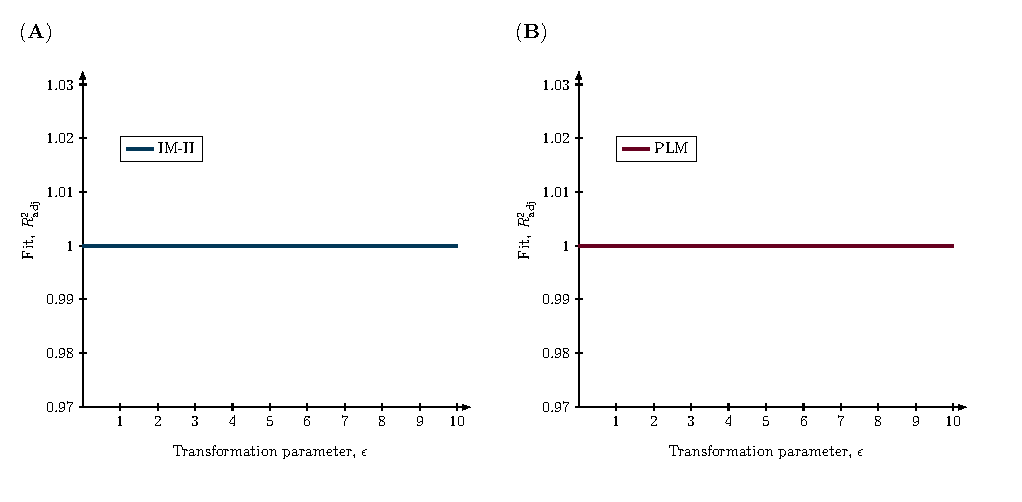
\includegraphics[width=\textwidth]{FigS5.pdf}
  \caption[Numerical validation of the symmetries]{\textit{Numerical validation of the symmetries}. The validation of the $t$-directional symmetries of the PLM and the IM-II is done in two steps. Firstly, each curve is transformed with a transformation parameter $\epsilon$. Secondly, the fit of the model to the the transformed data denoted by $R^2_{\mathrm{adj}}(\epsilon)$ is reported. In both cases, it is clear that $R^2_{\mathrm{adj}}\approx 1$ for all tested value of the transformation parameter $\epsilon$. The two tested symmetries are (\textbf{A}) $\Gamma_2$ for the IM-II and (\textbf{B}) $\Gamma_{1,1}$ for the PLM. The family of curves which these symmetries act on are defined by the parameters (\textbf{A}) $(\tau,\alpha)=(58.378,0.044)$ in the case of the IM-II and (\textbf{B}) $\gamma=4.528$ in the case of the PLM. The fit have been tested for multiple transformation parameters in the range $\epsilon\in [0,10]$. } 
  \label{fig:numerical_validation}
  \end{figure}



  The numerical validation of the $t$-directional symmetries of the PLM and the IM-II show that they are indeed symmetries. The fit of the models to the transformed solutions is $R^{2}_{\mathrm{adj}}(\epsilon)\approx 1$ (Fig \ref{fig:numerical_validation}) in both cases for a range of transformation parameters $\epsilon$. This illustrates that the scaling symmetry $\Gamma_{1,1}$ in the case of the PLM and the symmetry $\Gamma_{2}$ in case of the IM-II maps solution curves to other solution curves which is the defining property of a symmetry. 


%\section{Illustration of the symmetry based model selection for the PLM and the IM-II}

%\documentclass[tikz,crop,convert={density=200,outext=.png},border=0.4cm]{standalone}

\usepackage{pgfplots}
\usepackage{amsmath}
\usetikzlibrary{arrows.meta}
\usepackage{physics}
\usepackage{xcolor}
\definecolor{mixed_1}{RGB}{2,56,88}
\definecolor{mixed_2}{RGB}{54,144,192}
\definecolor{mixed_3}{RGB}{208,209,230}
\definecolor{pow_1}{RGB}{103,0,31}
\definecolor{pow_2}{RGB}{206,18,86}
\definecolor{pow_3}{RGB}{223,101,176}
\pgfplotsset{compat=newest,
    %width=6cm,
    %height=3cm,
    scale only axis=true,
    max space between ticks=25pt,
    try min ticks=5,
    every axis/.style={
        axis y line=middle,
        axis x line=middle,
        axis line style={thick,->,>=latex, shorten >=-.3cm}
    },
    every axis plot/.append style={thick},
    tick style={black, thick},
}
\tikzset{
    semithick/.style={line width=0.8pt},
}
\usepgfplotslibrary{groupplots}
\usepgfplotslibrary{dateplot}
% Document begins
\begin{document}
\begin{tikzpicture}
  % The axis of the plot
\begin{axis}[
    %title={Model: $\dv{y}{t}=\frac{2y}{t}$ with solution $y(t)=C_1t^2$\\Symmetry: $\Gamma_{\epsilon}=(t,y)\mapsto\left(\exp\left(\epsilon\right)t,\exp\left(-\epsilon\right)y\right)$},
    title style = {align=left},
    xlabel={Transformation parameter, $\epsilon$},
    ylabel={Adjusted $R^2$, $R^2_{\textrm{adj}}(\epsilon)$},
    %ylabel={Logarithm of Incidence, $\ln\left(R(t)\right)$},    
    % ylabel={Incidence, $R(t)$},
    x label style={at={(axis description cs:0.5,-0.1)},anchor=north},
    y label style={at={(axis description cs:-0.1,0.55)},rotate=90,anchor=south},    
    % xmin=-27, xmax=5,
    xmin=0, xmax=0.775,
    ymin = 0.83, ymax = 1.001,
    xtick={0,0.125,0.25,0.375,...,0.75},    
    %ymin=-14.5, ymax=1.5,
    %xtick={-30,-27,...,9},
    %ytick={1,0,-2,-4,-6,-8,-10,-12,-14},
    legend style={at={(axis description cs:0.05,0.7)},anchor=west},    
    %legend pos=north west,
    %ymajorgrids=true,
    grid style=dashed,
    x tick label style={
        /pgf/number format/.cd,
        fixed,
        fixed zerofill,
        precision=3,
        /tikz/.cd
    }
]    
]
% Plot the data
\addplot[
color=pow_1,line width=2pt,
]
coordinates {%
(0.0,1.0)
(0.10101010101010101,1.000000000000051)
(0.20202020202020202,0.999999999998303)
(0.30303030303030304,1.0000000000001539)
(0.40404040404040403,0.9999999999983028)
(0.5050505050505051,1.0000000000002565)
(0.6060606060606061,1.000000000000307)
(0.7070707070707071,0.999999999998303)
(0.8080808080808081,1.0000000000004097)
(0.9090909090909091,1.0000000000004612)
(1.0101010101010102,0.9999999999983027)
(1.1111111111111112,1.0000000000005638)
(1.2121212121212122,0.9999999999983029)
(1.3131313131313131,0.9999999999983028)
(1.4141414141414141,0.9999999999983028)
(1.5151515151515151,1.0000000000007685)
(1.6161616161616161,0.9999999999983029)
(1.7171717171717171,1.000000000000871)
(1.8181818181818181,0.9999999999983028)
(1.9191919191919191,1.0000000000009743)
(2.0202020202020203,1.0000000000010254)
(2.121212121212121,1.0000000000010765)
(2.2222222222222223,1.000000000001128)
(2.323232323232323,1.0000000000011795)
(2.4242424242424243,0.9999999999983029)
(2.525252525252525,0.9999999999983028)
(2.6262626262626263,1.0000000000013323)
(2.727272727272727,0.9999999999983029)
(2.8282828282828283,0.9999999999983028)
(2.929292929292929,0.9999999999983029)
(3.0303030303030303,0.9999999999983029)
(3.131313131313131,1.0000000000015896)
(3.2323232323232323,0.9999999999983029)
(3.3333333333333335,0.9999999999983028)
(3.4343434343434343,0.999999999998303)
(3.5353535353535355,1.0000000000017943)
(3.6363636363636362,1.0000000000018454)
(3.7373737373737375,1.0000000000018974)
(3.8383838383838382,1.0000000000019478)
(3.9393939393939394,1.0000000000019993)
(4.040404040404041,1.0000000000020506)
(4.141414141414141,0.9999999999983028)
(4.242424242424242,0.9999999999983029)
(4.343434343434343,0.9999999999983028)
(4.444444444444445,1.0000000000022569)
(4.545454545454545,1.0000000000023075)
(4.646464646464646,0.9999999999983028)
(4.747474747474747,0.9999999999983029)
(4.848484848484849,1.0000000000024623)
(4.94949494949495,1.000000000002512)
(5.05050505050505,0.999999999998303)
(5.151515151515151,1.0000000000026144)
(5.252525252525253,1.0000000000026665)
(5.353535353535354,1.000000000002718)
(5.454545454545454,0.9999999999983027)
(5.555555555555555,1.0000000000028204)
(5.656565656565657,1.0000000000028708)
(5.757575757575758,1.0000000000029228)
(5.858585858585858,0.9999999999983029)
(5.959595959595959,0.9999999999983027)
(6.0606060606060606,1.0000000000030764)
(6.161616161616162,1.0000000000031275)
(6.262626262626262,1.0000000000031783)
(6.363636363636363,1.0000000000032296)
(6.4646464646464645,1.000000000003282)
(6.565656565656566,1.0000000000033318)
(6.666666666666667,1.000000000003384)
(6.767676767676767,1.0000000000034348)
(6.8686868686868685,1.0000000000034859)
(6.96969696969697,0.9999999999983027)
(7.070707070707071,1.00000000000359)
(7.171717171717171,1.000000000003641)
(7.2727272727272725,1.0000000000036908)
(7.373737373737374,0.999999999998303)
(7.474747474747475,1.000000000003795)
(7.575757575757575,0.9999999999983027)
(7.6767676767676765,1.0000000000038956)
(7.777777777777778,0.9999999999983027)
(7.878787878787879,0.9999999999983029)
(7.979797979797979,1.0000000000040505)
(8.080808080808081,1.0000000000041016)
(8.181818181818182,1.0000000000041547)
(8.282828282828282,0.9999999999983031)
(8.383838383838384,0.9999999999983029)
(8.484848484848484,1.0000000000043072)
(8.585858585858587,1.0000000000043585)
(8.686868686868687,0.999999999998303)
(8.787878787878787,1.0000000000044604)
(8.88888888888889,0.9999999999983029)
(8.98989898989899,1.0000000000045648)
(9.09090909090909,1.000000000004614)
(9.191919191919192,1.0000000000046658)
(9.292929292929292,1.000000000004718)
(9.393939393939394,1.000000000004769)
(9.494949494949495,0.9999999999983032)
(9.595959595959595,1.0000000000048725)
(9.696969696969697,1.0000000000049225)
(9.797979797979798,1.0000000000049725)
(9.8989898989899,1.0000000000050229)
(10.0,1.0000000000050784)
};
\addlegendentry{PLM}
\addplot[
color=pow_1,line width=2pt,
]
coordinates {%
(0.0,1.0)
(0.10101010101010101,1.000000000000051)
(0.20202020202020202,0.999999999998303)
(0.30303030303030304,1.0000000000001539)
(0.40404040404040403,0.9999999999983028)
(0.5050505050505051,1.0000000000002565)
(0.6060606060606061,1.000000000000307)
(0.7070707070707071,0.999999999998303)
(0.8080808080808081,1.0000000000004097)
(0.9090909090909091,1.0000000000004612)
(1.0101010101010102,0.9999999999983027)
(1.1111111111111112,1.0000000000005638)
(1.2121212121212122,0.9999999999983029)
(1.3131313131313131,0.9999999999983028)
(1.4141414141414141,0.9999999999983028)
(1.5151515151515151,1.0000000000007685)
(1.6161616161616161,0.9999999999983029)
(1.7171717171717171,1.000000000000871)
(1.8181818181818181,0.9999999999983028)
(1.9191919191919191,1.0000000000009743)
(2.0202020202020203,1.0000000000010254)
(2.121212121212121,1.0000000000010765)
(2.2222222222222223,1.000000000001128)
(2.323232323232323,1.0000000000011795)
(2.4242424242424243,0.9999999999983029)
(2.525252525252525,0.9999999999983028)
(2.6262626262626263,1.0000000000013323)
(2.727272727272727,0.9999999999983029)
(2.8282828282828283,0.9999999999983028)
(2.929292929292929,0.9999999999983029)
(3.0303030303030303,0.9999999999983029)
(3.131313131313131,1.0000000000015896)
(3.2323232323232323,0.9999999999983029)
(3.3333333333333335,0.9999999999983028)
(3.4343434343434343,0.999999999998303)
(3.5353535353535355,1.0000000000017943)
(3.6363636363636362,1.0000000000018454)
(3.7373737373737375,1.0000000000018974)
(3.8383838383838382,1.0000000000019478)
(3.9393939393939394,1.0000000000019993)
(4.040404040404041,1.0000000000020506)
(4.141414141414141,0.9999999999983028)
(4.242424242424242,0.9999999999983029)
(4.343434343434343,0.9999999999983028)
(4.444444444444445,1.0000000000022569)
(4.545454545454545,1.0000000000023075)
(4.646464646464646,0.9999999999983028)
(4.747474747474747,0.9999999999983029)
(4.848484848484849,1.0000000000024623)
(4.94949494949495,1.000000000002512)
(5.05050505050505,0.999999999998303)
(5.151515151515151,1.0000000000026144)
(5.252525252525253,1.0000000000026665)
(5.353535353535354,1.000000000002718)
(5.454545454545454,0.9999999999983027)
(5.555555555555555,1.0000000000028204)
(5.656565656565657,1.0000000000028708)
(5.757575757575758,1.0000000000029228)
(5.858585858585858,0.9999999999983029)
(5.959595959595959,0.9999999999983027)
(6.0606060606060606,1.0000000000030764)
(6.161616161616162,1.0000000000031275)
(6.262626262626262,1.0000000000031783)
(6.363636363636363,1.0000000000032296)
(6.4646464646464645,1.000000000003282)
(6.565656565656566,1.0000000000033318)
(6.666666666666667,1.000000000003384)
(6.767676767676767,1.0000000000034348)
(6.8686868686868685,1.0000000000034859)
(6.96969696969697,0.9999999999983027)
(7.070707070707071,1.00000000000359)
(7.171717171717171,1.000000000003641)
(7.2727272727272725,1.0000000000036908)
(7.373737373737374,0.999999999998303)
(7.474747474747475,1.000000000003795)
(7.575757575757575,0.9999999999983027)
(7.6767676767676765,1.0000000000038956)
(7.777777777777778,0.9999999999983027)
(7.878787878787879,0.9999999999983029)
(7.979797979797979,1.0000000000040505)
(8.080808080808081,1.0000000000041016)
(8.181818181818182,1.0000000000041547)
(8.282828282828282,0.9999999999983031)
(8.383838383838384,0.9999999999983029)
(8.484848484848484,1.0000000000043072)
(8.585858585858587,1.0000000000043585)
(8.686868686868687,0.999999999998303)
(8.787878787878787,1.0000000000044604)
(8.88888888888889,0.9999999999983029)
(8.98989898989899,1.0000000000045648)
(9.09090909090909,1.000000000004614)
(9.191919191919192,1.0000000000046658)
(9.292929292929292,1.000000000004718)
(9.393939393939394,1.000000000004769)
(9.494949494949495,0.9999999999983032)
(9.595959595959595,1.0000000000048725)
(9.696969696969697,1.0000000000049225)
(9.797979797979798,1.0000000000049725)
(9.8989898989899,1.0000000000050229)
(10.0,1.0000000000050784)
};
\addlegendentry{PLM}
\addplot[
color=pow_1,line width=2pt,
]
coordinates {%
(0.0,1.0)
(0.10101010101010101,1.000000000000051)
(0.20202020202020202,0.999999999998303)
(0.30303030303030304,1.0000000000001539)
(0.40404040404040403,0.9999999999983028)
(0.5050505050505051,1.0000000000002565)
(0.6060606060606061,1.000000000000307)
(0.7070707070707071,0.999999999998303)
(0.8080808080808081,1.0000000000004097)
(0.9090909090909091,1.0000000000004612)
(1.0101010101010102,0.9999999999983027)
(1.1111111111111112,1.0000000000005638)
(1.2121212121212122,0.9999999999983029)
(1.3131313131313131,0.9999999999983028)
(1.4141414141414141,0.9999999999983028)
(1.5151515151515151,1.0000000000007685)
(1.6161616161616161,0.9999999999983029)
(1.7171717171717171,1.000000000000871)
(1.8181818181818181,0.9999999999983028)
(1.9191919191919191,1.0000000000009743)
(2.0202020202020203,1.0000000000010254)
(2.121212121212121,1.0000000000010765)
(2.2222222222222223,1.000000000001128)
(2.323232323232323,1.0000000000011795)
(2.4242424242424243,0.9999999999983029)
(2.525252525252525,0.9999999999983028)
(2.6262626262626263,1.0000000000013323)
(2.727272727272727,0.9999999999983029)
(2.8282828282828283,0.9999999999983028)
(2.929292929292929,0.9999999999983029)
(3.0303030303030303,0.9999999999983029)
(3.131313131313131,1.0000000000015896)
(3.2323232323232323,0.9999999999983029)
(3.3333333333333335,0.9999999999983028)
(3.4343434343434343,0.999999999998303)
(3.5353535353535355,1.0000000000017943)
(3.6363636363636362,1.0000000000018454)
(3.7373737373737375,1.0000000000018974)
(3.8383838383838382,1.0000000000019478)
(3.9393939393939394,1.0000000000019993)
(4.040404040404041,1.0000000000020506)
(4.141414141414141,0.9999999999983028)
(4.242424242424242,0.9999999999983029)
(4.343434343434343,0.9999999999983028)
(4.444444444444445,1.0000000000022569)
(4.545454545454545,1.0000000000023075)
(4.646464646464646,0.9999999999983028)
(4.747474747474747,0.9999999999983029)
(4.848484848484849,1.0000000000024623)
(4.94949494949495,1.000000000002512)
(5.05050505050505,0.999999999998303)
(5.151515151515151,1.0000000000026144)
(5.252525252525253,1.0000000000026665)
(5.353535353535354,1.000000000002718)
(5.454545454545454,0.9999999999983027)
(5.555555555555555,1.0000000000028204)
(5.656565656565657,1.0000000000028708)
(5.757575757575758,1.0000000000029228)
(5.858585858585858,0.9999999999983029)
(5.959595959595959,0.9999999999983027)
(6.0606060606060606,1.0000000000030764)
(6.161616161616162,1.0000000000031275)
(6.262626262626262,1.0000000000031783)
(6.363636363636363,1.0000000000032296)
(6.4646464646464645,1.000000000003282)
(6.565656565656566,1.0000000000033318)
(6.666666666666667,1.000000000003384)
(6.767676767676767,1.0000000000034348)
(6.8686868686868685,1.0000000000034859)
(6.96969696969697,0.9999999999983027)
(7.070707070707071,1.00000000000359)
(7.171717171717171,1.000000000003641)
(7.2727272727272725,1.0000000000036908)
(7.373737373737374,0.999999999998303)
(7.474747474747475,1.000000000003795)
(7.575757575757575,0.9999999999983027)
(7.6767676767676765,1.0000000000038956)
(7.777777777777778,0.9999999999983027)
(7.878787878787879,0.9999999999983029)
(7.979797979797979,1.0000000000040505)
(8.080808080808081,1.0000000000041016)
(8.181818181818182,1.0000000000041547)
(8.282828282828282,0.9999999999983031)
(8.383838383838384,0.9999999999983029)
(8.484848484848484,1.0000000000043072)
(8.585858585858587,1.0000000000043585)
(8.686868686868687,0.999999999998303)
(8.787878787878787,1.0000000000044604)
(8.88888888888889,0.9999999999983029)
(8.98989898989899,1.0000000000045648)
(9.09090909090909,1.000000000004614)
(9.191919191919192,1.0000000000046658)
(9.292929292929292,1.000000000004718)
(9.393939393939394,1.000000000004769)
(9.494949494949495,0.9999999999983032)
(9.595959595959595,1.0000000000048725)
(9.696969696969697,1.0000000000049225)
(9.797979797979798,1.0000000000049725)
(9.8989898989899,1.0000000000050229)
(10.0,1.0000000000050784)
};
\addlegendentry{PLM}
\addplot[
color=pow_1,line width=2pt,
]
coordinates {%
(0.0,1.0)
(0.10101010101010101,1.000000000000051)
(0.20202020202020202,0.999999999998303)
(0.30303030303030304,1.0000000000001539)
(0.40404040404040403,0.9999999999983028)
(0.5050505050505051,1.0000000000002565)
(0.6060606060606061,1.000000000000307)
(0.7070707070707071,0.999999999998303)
(0.8080808080808081,1.0000000000004097)
(0.9090909090909091,1.0000000000004612)
(1.0101010101010102,0.9999999999983027)
(1.1111111111111112,1.0000000000005638)
(1.2121212121212122,0.9999999999983029)
(1.3131313131313131,0.9999999999983028)
(1.4141414141414141,0.9999999999983028)
(1.5151515151515151,1.0000000000007685)
(1.6161616161616161,0.9999999999983029)
(1.7171717171717171,1.000000000000871)
(1.8181818181818181,0.9999999999983028)
(1.9191919191919191,1.0000000000009743)
(2.0202020202020203,1.0000000000010254)
(2.121212121212121,1.0000000000010765)
(2.2222222222222223,1.000000000001128)
(2.323232323232323,1.0000000000011795)
(2.4242424242424243,0.9999999999983029)
(2.525252525252525,0.9999999999983028)
(2.6262626262626263,1.0000000000013323)
(2.727272727272727,0.9999999999983029)
(2.8282828282828283,0.9999999999983028)
(2.929292929292929,0.9999999999983029)
(3.0303030303030303,0.9999999999983029)
(3.131313131313131,1.0000000000015896)
(3.2323232323232323,0.9999999999983029)
(3.3333333333333335,0.9999999999983028)
(3.4343434343434343,0.999999999998303)
(3.5353535353535355,1.0000000000017943)
(3.6363636363636362,1.0000000000018454)
(3.7373737373737375,1.0000000000018974)
(3.8383838383838382,1.0000000000019478)
(3.9393939393939394,1.0000000000019993)
(4.040404040404041,1.0000000000020506)
(4.141414141414141,0.9999999999983028)
(4.242424242424242,0.9999999999983029)
(4.343434343434343,0.9999999999983028)
(4.444444444444445,1.0000000000022569)
(4.545454545454545,1.0000000000023075)
(4.646464646464646,0.9999999999983028)
(4.747474747474747,0.9999999999983029)
(4.848484848484849,1.0000000000024623)
(4.94949494949495,1.000000000002512)
(5.05050505050505,0.999999999998303)
(5.151515151515151,1.0000000000026144)
(5.252525252525253,1.0000000000026665)
(5.353535353535354,1.000000000002718)
(5.454545454545454,0.9999999999983027)
(5.555555555555555,1.0000000000028204)
(5.656565656565657,1.0000000000028708)
(5.757575757575758,1.0000000000029228)
(5.858585858585858,0.9999999999983029)
(5.959595959595959,0.9999999999983027)
(6.0606060606060606,1.0000000000030764)
(6.161616161616162,1.0000000000031275)
(6.262626262626262,1.0000000000031783)
(6.363636363636363,1.0000000000032296)
(6.4646464646464645,1.000000000003282)
(6.565656565656566,1.0000000000033318)
(6.666666666666667,1.000000000003384)
(6.767676767676767,1.0000000000034348)
(6.8686868686868685,1.0000000000034859)
(6.96969696969697,0.9999999999983027)
(7.070707070707071,1.00000000000359)
(7.171717171717171,1.000000000003641)
(7.2727272727272725,1.0000000000036908)
(7.373737373737374,0.999999999998303)
(7.474747474747475,1.000000000003795)
(7.575757575757575,0.9999999999983027)
(7.6767676767676765,1.0000000000038956)
(7.777777777777778,0.9999999999983027)
(7.878787878787879,0.9999999999983029)
(7.979797979797979,1.0000000000040505)
(8.080808080808081,1.0000000000041016)
(8.181818181818182,1.0000000000041547)
(8.282828282828282,0.9999999999983031)
(8.383838383838384,0.9999999999983029)
(8.484848484848484,1.0000000000043072)
(8.585858585858587,1.0000000000043585)
(8.686868686868687,0.999999999998303)
(8.787878787878787,1.0000000000044604)
(8.88888888888889,0.9999999999983029)
(8.98989898989899,1.0000000000045648)
(9.09090909090909,1.000000000004614)
(9.191919191919192,1.0000000000046658)
(9.292929292929292,1.000000000004718)
(9.393939393939394,1.000000000004769)
(9.494949494949495,0.9999999999983032)
(9.595959595959595,1.0000000000048725)
(9.696969696969697,1.0000000000049225)
(9.797979797979798,1.0000000000049725)
(9.8989898989899,1.0000000000050229)
(10.0,1.0000000000050784)
};
\addlegendentry{PLM}

% Plot the model
\addplot[
color=mixed_1,line width=2pt,
]
coordinates {%
(0.0,1.0)
(0.10101010101010101,1.0012043532805712)
(0.20202020202020202,1.0023505723923285)
(0.30303030303030304,1.0034356241007256)
(0.40404040404040403,1.0044563206081527)
(0.5050505050505051,1.0054093105940847)
(0.6060606060606061,1.0062910696338552)
(0.7070707070707071,1.007097889982874)
(0.8080808080808081,1.0078258696719316)
(0.9090909090909091,1.008470900832512)
(1.0101010101010102,1.00902865721923)
(1.1111111111111112,1.0094945808622393)
(1.2121212121212122,1.0098638677509362)
(1.3131313131313131,1.0101314525216283)
(1.4141414141414141,1.0102919920147964)
(1.5151515151515151,1.0103398476395578)
(1.6161616161616161,1.0102690664336977)
(1.7171717171717171,1.0100733607144166)
(1.8181818181818181,1.0097460861811556)
(1.9191919191919191,1.0092802183762342)
(2.0202020202020203,1.0086683272971229)
(2.121212121212121,1.0079025500617318)
(2.2222222222222223,1.0069745614013483)
(2.323232323232323,1.0058755418178462)
(2.4242424242424243,1.0045961431578874)
(2.525252525252525,1.003126451400547)
(2.6262626262626263,1.0014559463639097)
(2.727272727272727,0.9995734580542746)
(2.8282828282828283,0.9974671193283466)
(2.929292929292929,0.9951243145086941)
(3.0303030303030303,0.9925316235518113)
(3.131313131313131,0.9896747613227708)
(3.2323232323232323,0.9865385114820413)
(3.3333333333333335,0.9831066544160483)
(3.4343434343434343,0.979361888609222)
(3.5353535353535355,0.9752857447851875)
(3.6363636363636362,0.970858491938326)
(3.7373737373737375,0.9660590345050339)
(3.8383838383838382,0.9608647997109221)
(3.9393939393939394,0.955251613617643)
(4.040404040404041,0.9491935654128263)
(4.141414141414141,0.942662857502936)
(4.242424242424242,0.93562964088632)
(4.343434343434343,0.9280618327636733)
(4.444444444444445,0.9199249156966254)
(4.545454545454545,0.9111817149187648)
(4.646464646464646,0.9017921515312413)
(4.747474747474747,0.8917129684659207)
(4.848484848484849,0.8808974257615754)
(4.94949494949495,0.8692949610423103)
(5.05050505050505,0.8568508106010593)
(5.151515151515151,0.8435055857318593)
(5.252525252525253,0.829194798124276)
(5.353535353535354,0.8138483271468511)
(5.454545454545454,0.7973898206814479)
(5.555555555555555,0.7797360197891691)
(5.656565656565657,0.76079599575332)
(5.757575757575758,0.7404702868362778)
(5.858585858585858,0.7186499171216443)
(5.959595959595959,0.6952152822597837)
(6.0606060606060606,0.670034876868451)
(6.161616161616162,0.6429638397018237)
(6.262626262626262,0.6138422858767353)
(6.363636363636363,0.582493385432634)
(6.4646464646464645,0.5487211501921313)
(6.565656565656566,0.5123078720973638)
(6.666666666666667,0.4730111407735748)
(6.767676767676767,0.43056037580593576)
(6.8686868686868685,0.3846527716208117)
(6.96969696969697,0.33494852364421335)
(7.070707070707071,0.28106521046313654)
(7.171717171717171,0.22257113613831284)
(7.2727272727272725,0.15897741075842162)
(7.373737373737374,0.08972848402635714)
(7.474747474747475,0.014190772170601456)
(7.575757575757575,-0.06836108008120839)
(7.6767676767676765,-0.1587608842275779)
(7.777777777777778,-0.25797131013716224)
(7.878787878787879,-0.36710896815469024)
(7.979797979797979,-0.48747548672230157)
(8.080808080808081,-0.6205962843846058)
(8.181818181818182,-0.7682693377479362)
(8.282828282828282,-0.9326270231355369)
(8.383838383838384,-1.116215307104148)
(8.484848484848484,-1.3220960851803347)
(8.585858585858587,-1.5539809361948602)
(8.686868686868687,-1.8164079389258496)
(8.787878787878787,-2.1149784215365894)
(8.88888888888889,-2.4566784039919902)
(8.98989898989899,-2.8503217684361695)
(9.09090909090909,-3.3071716879225765)
(9.191919191919192,-3.841828552040901)
(9.292929292929292,-4.473525598906787)
(9.393939393939394,-5.228064600897703)
(9.494949494949495,-6.140786065604821)
(9.595959595959595,-7.2612678327702245)
(9.696969696969697,-8.66102316977074)
(9.797979797979798,-10.446638588964774)
(9.8989898989899,-12.783299836264067)
(10.0,-15.939414411582948)
};
\addlegendentry{IM-II}
\addplot[
color=mixed_1,line width=2pt,
]
coordinates {%
(0.0,1.0)
(0.10101010101010101,1.0011842396146424)
(0.20202020202020202,1.0023113159477255)
(0.30303030303030304,1.003378246422154)
(0.40404040404040403,1.0043818964790945)
(0.5050505050505051,1.0053189707677639)
(0.6060606060606061,1.0061860037242147)
(0.7070707070707071,1.0069793495261663)
(0.8080808080808081,1.0076951713704245)
(0.9090909090909091,1.0083294299931729)
(1.0101010101010102,1.0088778714007955)
(1.1111111111111112,1.0093360137451983)
(1.2121212121212122,1.0096991332466085)
(1.3131313131313131,1.009962249136971)
(1.4141414141414141,1.010120107491817)
(1.5151515151515151,1.0101671638892546)
(1.6161616161616161,1.0100975647863137)
(1.7171717171717171,1.0099051275095416)
(1.8181818181818181,1.0095833187235286)
(1.9191919191919191,1.009125231284673)
(2.0202020202020203,1.0085235592774477)
(2.121212121212121,1.007770571136201)
(2.2222222222222223,1.0068580806308876)
(2.323232323232323,1.0057774155560735)
(2.4242424242424243,1.0045193838800817)
(2.525252525252525,1.0030742371540893)
(2.6262626262626263,1.0014316308916587)
(2.727272727272727,0.9995805816469442)
(2.8282828282828283,0.9975094204674639)
(2.929292929292929,0.9952057423677196)
(3.0303030303030303,0.9926563514296977)
(3.131313131313131,0.9898472010916838)
(3.2323232323232323,0.9867633291392234)
(3.3333333333333335,0.9833887868393003)
(3.4343434343434343,0.9797065616255343)
(3.5353535353535355,0.9756984926732819)
(3.6363636363636362,0.9713451785005467)
(3.7373737373737375,0.9666258758565602)
(3.8383838383838382,0.9615183889503739)
(3.9393939393939394,0.9559989475678029)
(4.040404040404041,0.9500420736278298)
(4.141414141414141,0.9436204337790296)
(4.242424242424242,0.9367046775220232)
(4.343434343434343,0.9292632578659914)
(4.444444444444445,0.9212622338414743)
(4.545454545454545,0.9126650515304814)
(4.646464646464646,0.9034323013839254)
(4.747474747474747,0.8935214487614106)
(4.848484848484849,0.8828865342965574)
(4.94949494949495,0.8714778400457098)
(5.05050505050505,0.8592415168996418)
(5.151515151515151,0.8461191679914218)
(5.252525252525253,0.8320473820171329)
(5.353535353535354,0.8169572094161138)
(5.454545454545454,0.8007735732118507)
(5.555555555555555,0.7834146049565174)
(5.656565656565657,0.7647908945159315)
(5.757575757575758,0.744804641243278)
(5.858585858585858,0.7233486892073837)
(5.959595959595959,0.7003054315471998)
(6.0606060606060606,0.6755455591258593)
(6.161616161616162,0.6489266299965543)
(6.262626262626262,0.620291429481928)
(6.363636363636363,0.5894660808236245)
(6.4646464646464645,0.5562578690040417)
(6.565656565656566,0.5204527218645294)
(6.666666666666667,0.48181227747805366)
(6.767676767676767,0.4400704743397753)
(6.8686868686868685,0.39492956397205264)
(6.96969696969697,0.3460554168098766)
(7.070707070707071,0.2930719981846222)
(7.171717171717171,0.23555482182551712)
(7.2727272727272725,0.17302316267495219)
(7.373737373737374,0.10493074857145059)
(7.474747474747475,0.03065457710074576)
(7.575757575757575,-0.05051859299459004)
(7.6767676767676765,-0.13940864789214596)
(7.777777777777778,-0.23696218010150738)
(7.878787878787879,-0.34427715167889167)
(7.979797979797979,-0.4626334528272757)
(8.080808080808081,-0.5935310263778689)
(8.181818181818182,-0.7387378212853255)
(8.282828282828282,-0.9003506014776791)
(8.383838383838384,-1.0808728138277741)
(8.484848484848484,-1.2833152177506006)
(8.585858585858587,-1.5113274057329846)
(8.686868686868687,-1.7693716669969677)
(8.787878787878787,-2.062955783032071)
(8.88888888888889,-2.3989491016655413)
(8.98989898989899,-2.78601830613911)
(9.09090909090909,-3.2352384654808106)
(9.191919191919192,-3.7609661310616174)
(9.292929292929292,-4.382113330491555)
(9.393939393939394,-5.124050925850971)
(9.494949494949495,-6.021529209903775)
(9.595959595959595,-7.12329803269655)
(9.696969696969697,-8.499676332672319)
(9.797979797979798,-10.255470541928407)
(9.8989898989899,-12.553107671906268)
(10.0,-15.65651260195266)
};
\addlegendentry{IM-II}
\addplot[
color=mixed_1,line width=2pt,
]
coordinates {%
(0.0,1.0)
(0.10101010101010101,1.0011842396146424)
(0.20202020202020202,1.0023113159477255)
(0.30303030303030304,1.003378246422154)
(0.40404040404040403,1.0043818964790945)
(0.5050505050505051,1.0053189707677639)
(0.6060606060606061,1.0061860037242147)
(0.7070707070707071,1.0069793495261663)
(0.8080808080808081,1.0076951713704245)
(0.9090909090909091,1.0083294299931729)
(1.0101010101010102,1.0088778714007955)
(1.1111111111111112,1.0093360137451983)
(1.2121212121212122,1.0096991332466085)
(1.3131313131313131,1.009962249136971)
(1.4141414141414141,1.010120107491817)
(1.5151515151515151,1.0101671638892546)
(1.6161616161616161,1.0100975647863137)
(1.7171717171717171,1.0099051275095416)
(1.8181818181818181,1.0095833187235286)
(1.9191919191919191,1.009125231284673)
(2.0202020202020203,1.0085235592774477)
(2.121212121212121,1.007770571136201)
(2.2222222222222223,1.0068580806308876)
(2.323232323232323,1.0057774155560735)
(2.4242424242424243,1.0045193838800817)
(2.525252525252525,1.0030742371540893)
(2.6262626262626263,1.0014316308916587)
(2.727272727272727,0.9995805816469442)
(2.8282828282828283,0.9975094204674639)
(2.929292929292929,0.9952057423677196)
(3.0303030303030303,0.9926563514296977)
(3.131313131313131,0.9898472010916838)
(3.2323232323232323,0.9867633291392234)
(3.3333333333333335,0.9833887868393003)
(3.4343434343434343,0.9797065616255343)
(3.5353535353535355,0.9756984926732819)
(3.6363636363636362,0.9713451785005467)
(3.7373737373737375,0.9666258758565602)
(3.8383838383838382,0.9615183889503739)
(3.9393939393939394,0.9559989475678029)
(4.040404040404041,0.9500420736278298)
(4.141414141414141,0.9436204337790296)
(4.242424242424242,0.9367046775220232)
(4.343434343434343,0.9292632578659914)
(4.444444444444445,0.9212622338414743)
(4.545454545454545,0.9126650515304814)
(4.646464646464646,0.9034323013839254)
(4.747474747474747,0.8935214487614106)
(4.848484848484849,0.8828865342965574)
(4.94949494949495,0.8714778400457098)
(5.05050505050505,0.8592415168996418)
(5.151515151515151,0.8461191679914218)
(5.252525252525253,0.8320473820171329)
(5.353535353535354,0.8169572094161138)
(5.454545454545454,0.8007735732118507)
(5.555555555555555,0.7834146049565174)
(5.656565656565657,0.7647908945159315)
(5.757575757575758,0.744804641243278)
(5.858585858585858,0.7233486892073837)
(5.959595959595959,0.7003054315471998)
(6.0606060606060606,0.6755455591258593)
(6.161616161616162,0.6489266299965543)
(6.262626262626262,0.620291429481928)
(6.363636363636363,0.5894660808236245)
(6.4646464646464645,0.5562578690040417)
(6.565656565656566,0.5204527218645294)
(6.666666666666667,0.48181227747805366)
(6.767676767676767,0.4400704743397753)
(6.8686868686868685,0.39492956397205264)
(6.96969696969697,0.3460554168098766)
(7.070707070707071,0.2930719981846222)
(7.171717171717171,0.23555482182551712)
(7.2727272727272725,0.17302316267495219)
(7.373737373737374,0.10493074857145059)
(7.474747474747475,0.03065457710074576)
(7.575757575757575,-0.05051859299459004)
(7.6767676767676765,-0.13940864789214596)
(7.777777777777778,-0.23696218010150738)
(7.878787878787879,-0.34427715167889167)
(7.979797979797979,-0.4626334528272757)
(8.080808080808081,-0.5935310263778689)
(8.181818181818182,-0.7387378212853255)
(8.282828282828282,-0.9003506014776791)
(8.383838383838384,-1.0808728138277741)
(8.484848484848484,-1.2833152177506006)
(8.585858585858587,-1.5113274057329846)
(8.686868686868687,-1.7693716669969677)
(8.787878787878787,-2.062955783032071)
(8.88888888888889,-2.3989491016655413)
(8.98989898989899,-2.78601830613911)
(9.09090909090909,-3.2352384654808106)
(9.191919191919192,-3.7609661310616174)
(9.292929292929292,-4.382113330491555)
(9.393939393939394,-5.124050925850971)
(9.494949494949495,-6.021529209903775)
(9.595959595959595,-7.12329803269655)
(9.696969696969697,-8.499676332672319)
(9.797979797979798,-10.255470541928407)
(9.8989898989899,-12.553107671906268)
(10.0,-15.65651260195266)
};
\addlegendentry{IM-II}
\addplot[
color=mixed_1,line width=2pt,
]
coordinates {%
(0.0,1.0)
(0.10101010101010101,1.0011842396146424)
(0.20202020202020202,1.0023113159477255)
(0.30303030303030304,1.003378246422154)
(0.40404040404040403,1.0043818964790945)
(0.5050505050505051,1.0053189707677639)
(0.6060606060606061,1.0061860037242147)
(0.7070707070707071,1.0069793495261663)
(0.8080808080808081,1.0076951713704245)
(0.9090909090909091,1.0083294299931729)
(1.0101010101010102,1.0088778714007955)
(1.1111111111111112,1.0093360137451983)
(1.2121212121212122,1.0096991332466085)
(1.3131313131313131,1.009962249136971)
(1.4141414141414141,1.010120107491817)
(1.5151515151515151,1.0101671638892546)
(1.6161616161616161,1.0100975647863137)
(1.7171717171717171,1.0099051275095416)
(1.8181818181818181,1.0095833187235286)
(1.9191919191919191,1.009125231284673)
(2.0202020202020203,1.0085235592774477)
(2.121212121212121,1.007770571136201)
(2.2222222222222223,1.0068580806308876)
(2.323232323232323,1.0057774155560735)
(2.4242424242424243,1.0045193838800817)
(2.525252525252525,1.0030742371540893)
(2.6262626262626263,1.0014316308916587)
(2.727272727272727,0.9995805816469442)
(2.8282828282828283,0.9975094204674639)
(2.929292929292929,0.9952057423677196)
(3.0303030303030303,0.9926563514296977)
(3.131313131313131,0.9898472010916838)
(3.2323232323232323,0.9867633291392234)
(3.3333333333333335,0.9833887868393003)
(3.4343434343434343,0.9797065616255343)
(3.5353535353535355,0.9756984926732819)
(3.6363636363636362,0.9713451785005467)
(3.7373737373737375,0.9666258758565602)
(3.8383838383838382,0.9615183889503739)
(3.9393939393939394,0.9559989475678029)
(4.040404040404041,0.9500420736278298)
(4.141414141414141,0.9436204337790296)
(4.242424242424242,0.9367046775220232)
(4.343434343434343,0.9292632578659914)
(4.444444444444445,0.9212622338414743)
(4.545454545454545,0.9126650515304814)
(4.646464646464646,0.9034323013839254)
(4.747474747474747,0.8935214487614106)
(4.848484848484849,0.8828865342965574)
(4.94949494949495,0.8714778400457098)
(5.05050505050505,0.8592415168996418)
(5.151515151515151,0.8461191679914218)
(5.252525252525253,0.8320473820171329)
(5.353535353535354,0.8169572094161138)
(5.454545454545454,0.8007735732118507)
(5.555555555555555,0.7834146049565174)
(5.656565656565657,0.7647908945159315)
(5.757575757575758,0.744804641243278)
(5.858585858585858,0.7233486892073837)
(5.959595959595959,0.7003054315471998)
(6.0606060606060606,0.6755455591258593)
(6.161616161616162,0.6489266299965543)
(6.262626262626262,0.620291429481928)
(6.363636363636363,0.5894660808236245)
(6.4646464646464645,0.5562578690040417)
(6.565656565656566,0.5204527218645294)
(6.666666666666667,0.48181227747805366)
(6.767676767676767,0.4400704743397753)
(6.8686868686868685,0.39492956397205264)
(6.96969696969697,0.3460554168098766)
(7.070707070707071,0.2930719981846222)
(7.171717171717171,0.23555482182551712)
(7.2727272727272725,0.17302316267495219)
(7.373737373737374,0.10493074857145059)
(7.474747474747475,0.03065457710074576)
(7.575757575757575,-0.05051859299459004)
(7.6767676767676765,-0.13940864789214596)
(7.777777777777778,-0.23696218010150738)
(7.878787878787879,-0.34427715167889167)
(7.979797979797979,-0.4626334528272757)
(8.080808080808081,-0.5935310263778689)
(8.181818181818182,-0.7387378212853255)
(8.282828282828282,-0.9003506014776791)
(8.383838383838384,-1.0808728138277741)
(8.484848484848484,-1.2833152177506006)
(8.585858585858587,-1.5113274057329846)
(8.686868686868687,-1.7693716669969677)
(8.787878787878787,-2.062955783032071)
(8.88888888888889,-2.3989491016655413)
(8.98989898989899,-2.78601830613911)
(9.09090909090909,-3.2352384654808106)
(9.191919191919192,-3.7609661310616174)
(9.292929292929292,-4.382113330491555)
(9.393939393939394,-5.124050925850971)
(9.494949494949495,-6.021529209903775)
(9.595959595959595,-7.12329803269655)
(9.696969696969697,-8.499676332672319)
(9.797979797979798,-10.255470541928407)
(9.8989898989899,-12.553107671906268)
(10.0,-15.65651260195266)
};
\addlegendentry{IM-II}

\end{axis}
\end{tikzpicture}

\end{document}



\newpage
\bibliography{model_selection_symmetries_cancer} 
\bibliographystyle{ieeetr}

% THE DOCUMENT ENDS
\end{document}
